\documentclass[bibtotoc,liststotoc,BCOR=5mm,DIV=12]{scrbook}

% use this declaration to set specific page margins
%\usepackage[a4paper , lmargin = {2.7cm} , rmargin = {2.9cm} , tmargin = {2.7cm} , bmargin = {4.6cm} ]{geometry}
\usepackage[a4paper]{geometry}

\usepackage[ngerman, english]{babel}
\usepackage{bibgerm}       		% german references
\usepackage[T1]{fontenc} % german characters
\usepackage{graphicx} 				% it's recommended to use PDF images but you can use JPG or PNG as well
\usepackage{url}           		% format URLs
\usepackage{hyperref} 				% create hyperlinks
\usepackage{listings, color}	% for source code
\usepackage{subfig}						% two figures next to each other (example: figure 3a), figure 3b)
\usepackage{scrlayer-scrpage}					% header and footer line
\usepackage{todonotes}
\usepackage{cleveref}
% header and footer line - no header & footer line on pages where a new chapter starts
\pagestyle{scrheadings}
\ohead{Design and Implementation of Content Provenance\\using C2PA Signatures in Live Streaming}
\ihead{Philip Nys}
\ofoot[]{\thepage}
\ifoot{Master's Thesis, TU Berlin, Fachgebiet ODS, 2025}

% set path where images are stored
\graphicspath{{./img/}}

%
% der Befehl \hypenation versteht keine Sonderzeichen, also weder ä
% noch "a noch \"a. Wörter die derartige Zeichen enthalten müssen
% direkt im Text getrennt werden, z.B. Wör\-ter
%
\hyphenation{te-le-com-muni-cation 
te-le-com-muni-cation-specific 
Te-le-kom-mu-ni-ka-tions-API} 					% use this file to set explicit hyphenations (doesn't seem to work correctly)

\begin{document}
% ---------------------------------------------------------------
\frontmatter
    \thispagestyle{empty}
\begin{center}

\vspace*{1.4cm}
{\LARGE \textbf{Technische Universität Berlin}}

\vspace{0.5cm}

{\large Open Distributed Systems\\[1mm]}

Fakultät IV\\
Einsteinufer 25\\
10587 Berlin\\
https://www.tu.berlin/ods\\

\vspace*{1cm}


\includegraphics[width=4cm]{tu_logo}

\vspace*{1.0cm}

{\LARGE Master's Thesis}\\

\vspace{1.0cm}
{\LARGE \textbf{Design and Implementation}}\\
\vspace*{0.3cm}
{\LARGE \textbf{of Content Provenance using C2PA Signatures in Live Streaming}}\\
\vspace*{1.0cm}
{\LARGE Philip Nys}
\\
\vspace*{0.5cm}
Matriculation Number: 397914\\
09.07.2025\\ % 	date of submission
\vspace*{1.0cm}

Supervised by\\
Prof. Dr. Manfred Hauswirth\\
Prof. Dr. Volker Markl

\vspace*{0.5cm}
Assistant Supervisor\\
Stefan Pham\\
\vspace{3cm}


\end{center}


    \thispagestyle{empty}
    \cleardoublepage
    
    
    \newpage

\thispagestyle{empty}

\begin{large}

\vspace*{6cm}

\noindent
Hereby I declare that I wrote this thesis myself with the help of no more than the mentioned literature and auxiliary means.
\vspace{2cm}

\noindent
Berlin, \today

\vspace{3cm}

\hspace*{7cm}%
\dotfill\\
\hspace*{8.5cm}%
\textit{(Philip Nys)}

\end{large}
 
    \thispagestyle{empty}
    \cleardoublepage
    
    
    \thispagestyle{empty}
\vspace*{1.0cm}

\begin{center}
    \textbf{Abstract}
\end{center}

\vspace*{0.5cm}

\noindent

It is getting more and more difficult to trust the media you see on the internet. The tools for editing, manipulating, creating and generating media are getting easier to use and more accessible every day.

There are tools, like image filters on social media, which essentially require no expertise to use at all, but also highly specialized tools for manipulating all kinds of media, like images, videos, audio, documents and more, with results that make it harder than ever to distinguish real from forged.

Additionally, there are also now a plethora of tools that are able to generated these kinds of media from just a single text prompt. The results of which are getting more and more convincing as these tools are being iterated upon.

All of this is creating new problems in society, like false perceptions of beauty, unbelievable documentations, faking personalities and content to scam people and many more.

This has lead to the founding of the Coalition of Content Provenance and Authenticity (C2PA) by large companies in the industry. Their goal is to create a standard of embedding metadata into all kinds of data types to document the road media took from creation to the consumption and spread its use to as many places as possible. This metadata is to detail everything involved in the creation, editing, distribution and anything else relevant of the corresponding media.

This data should provide users the option to inform themselves whether the media they are viewing is from a trustworthy source or perhaps may have been tampered with or is from a nefarious source.

    \thispagestyle{empty}
    \cleardoublepage
    
    \thispagestyle{empty}
\vspace*{0.2cm}

\begin{center}
    \textbf{Zusammenfassung}
\end{center}

\vspace*{0.2cm}

\noindent 

Es wird immer schwieriger Media im Internet zu vertrauen. Die Programme zum Bearbeiten, Manipulieren, Erstellen und Generierung von Media werden jeden Tag leichter zu bedienen.

Es gibt Programme, wie zum Bespiel Bildfilter in Soziel Medien, welche praktisch kein Vorwissen benötigen, aber auch hochspezialisierte Programme zur Bearbeitung von jeglichen Arten von Media, wie Bilder, Videos, Audio, Dokumente und mehr, mit Ergebnissen, welche schwerer denn je sind, echten Inhalt von Gefälschten zu unterscheiden.

Dazu kommen zahlreiche Programme, welche in der Lage sind diese Arten von Medien aus nur einer einfachen Textaufforderung zu erzeugen. Deren Ergebnisse mit der Zeit immer überzeugender werden, da sich diese Programma stetig verbessern.

All das führt zu neuen Problem in der Gesellschaft, wie zum Bespiel eine falsche Vorstellung von Schönheit, unglaubwürdigen Dokumenten, Identitätsraub und gefälschten Inhalten, welche verwendet werden, um Leute zu täuschen und auszurauben und Vieles mehr.

Dies hat zu der Gründung der Coalition of Content Provenance and Authenticity (C2PA), das Bündnis für Inhaltsherkunft und -authentizität, durch großen Unternehmen aus der Industrie geführt. Dessen Ziel ist es einen Standart zu entwicklen, welcher Eckdaten in all möglichen Datentypen einzubetten. Diese Daten sollen alle Schritten dokumentieren, die dieser Datentyp von Erstellung bis hin zum Endnutzer durchlaufen ist. Dies schließt jedes Detail ein, welche bei der Erstellung, Bearbeitung, Verteilung und jegliche weitere Information beigetragen haben.

Diesen Daten ermöglichen den Endnutzern die Option sich selbst für den Entstehungsweg des entsprechenden Mediums zu informieren und sicher stellen, dass Dies aus einer vertrauenwürdigen Quelle kommt oder manipuliert wurde oder möglicherweise eine schädlichen Ursprung hat.
    \thispagestyle{empty}
    
    
    \tableofcontents
    \thispagestyle{empty}
    
    \todo[inline]{talk to your supervisor if this is needed}
    \listoffigures
    \thispagestyle{empty}
    
    \listoftables
    \thispagestyle{empty}
    
% --------------------------------------------------------------

\mainmatter % comment single chapters for faster compilation

    \chapter{Introduction\label{cha:chapter1}}

\section{Motivation\label{sec:moti}}

For millennia human beings have been forging documents, paintings, photographs, videos and any other type of media, ranging from analog manipulations, like altering shipping manifests on clay tablets, duplicating paintings and altering the development of photos and films, to digital tools with varying levels of difficulties, from complex tools like PhotoShop, GIMP and Photopea for images, AfterEffects, Blender and Nuke for videos, to easy tools like image filters on social media.

In this digital age, these tools are not only getting more accessible, but also easier to use, while delivering results better than ever. This has the consequence that it is getting more difficult to discern real media from manipulated media, especially for people that are less familiar with these tools.

To make things worse, in the past few years many new tools have been released that are capable of generating new media from just a simple text prompt. Large Language Models (LLMs), like ChatGPT, Gemini and DeepSeek, are capable of generating texts, like essays, articles and more. There are also image generators, like Midjourney, Stable Diffusion and Firefly, as well as Sora, Synthesia and Capsule for videos. The list of these tools grows steadily every day, with numerous additional application types: music generation, voice cloning, face replacements and many more.

All this has lead to the founding of the Coalition for Content Provenance and Authenticity (C2PA) by Adobe, Arm, BBC, Intel, Microsoft and Truepic on February 22nd, 2021 \footnote{C2PA Founding Press Release: \url{https://c2pa.org/post/c2pa_initial_pr/}}. The ultimate goal of C2PA is the development and integration of a taper-proof manifest into digital media, which protocol all steps it has gone through from its creation to the present, as well as the tools, people, devices and locations involved and any additional relevant metadata. This allows everyone interacting with C2PA-signed media to verify that that media is trustworthy and look at the metadata and potentially see that it has been automatically generated, edited, applied with a filter or anything else.

At the writing of this thesis there is no specifications in regards to applying C2PA to live streaming and there is also not much material about other people researching into this topic. This thesis will be filling in this gap by implementing and evaluating C2PA in a live streaming context.

\section{Objective\label{sec:objective}}

The current version 2.1 of the C2PA technical specification \footnote{C2PA Technical Specification \url{https://c2pa.org/specifications/specifications/2.1/specs/C2PA_Specification.html}} has no explicit specifications for live streaming content and there are currently no public discussions or proof-of-concepts on how C2PA signing should work when live streaming media. There is, however, a specification with a working implementation for fragmented BMFF (Base Media File Format) media.

This thesis will describe and evaluate a proof-of-concept of adapting the existing fragmented BMFF implementation to a live streaming testbed compliant with the DASH and HLS streaming protocols. In addition to this, it will also propose an alternative approach that is specifically catered to live streaming.

\section{Scope\label{sec:scope}}

The aforementioned proof-of-concept is a live streaming testbed which will roughly emulate a real-world scenario. It consists of four components.

The first component is Producer and its tasks is to create a DASH and HLS live stream. That live stream is then forwarded to the Signer, which will sign the live stream with a C2PA manifest. From there the signed live stream is published to the CDN (content delivery network), which will host the live stream and make it available for consumption. Finally, the Consumer will request the live stream from the CDN, play it back and also validate that the received live stream is trustworthy based on the embedded C2PA manifest. This testbed is visualized in \Cref{fig:testbed}.

\begin{figure}[H]
    \centering
    \begin{tikzpicture}[node distance=2cm]
        \node (producer) [component] {Producer};
        \node (c2pa) [component, above of=producer, yshift=1cm] {Signer};
        \node (cdn) [component, right of=c2pa, xshift=3.5cm] {CDN};
        \node (consumer) [component, below of=cdn, yshift=-1cm] {Consumer};
    
        \draw [arrow] (producer) -- node[anchor=east, text width=2cm, text centered, xshift=0.15cm] {create MPEG-DASH / HLS stream} (c2pa);
        \draw [arrow] (c2pa) -- node[anchor=south, text width=2cm, text centered] {publish signed segments} (cdn);
        \draw [arrow] (consumer) -- node[anchor=east, text width=2cm, text centered, xshift=0.4cm] {request stream} (cdn);
        \draw [arrow] (cdn) -- node[anchor=west, text width=2cm, text centered, xshift=-0.4cm] {provide stream} (consumer);
    \end{tikzpicture}
    \caption{Proof of Concept Testbed Setup}
    \label{fig:testbed}
\end{figure}

\section{Outline\label{sec:outline}}

The remaining thesis is structured into the following chapters:
\\
\\
\textbf{Chapter \ref{cha:chapter2}} will describe the State of the Art with a introduction to HTTP Adaptive Streaming (HAS), an in-depth overview of C2PA as well as concurrent live streaming approaches.
\\
\\
\textbf{Chapter \ref{cha:chapter3}} will list the requirements of this thesis and its implementation.
\\
\\
\textbf{Chapter \ref{cha:chapter4}} will go over the design of the testbed, including details of the four components.
\\
\\
\textbf{Chapter \ref{cha:chapter5}} will outline specific technical aspects of the implementation.
\\
\\
\textbf{Chapter \ref{cha:chapter6}} will evaluate C2PA in a live streaming scenario as part of this proof-of-concept.
\\
\\
\textbf{Chapter \ref{cha:chapter7}} will conclude this thesis with a summary, dissemination and an outlook to possible further research.
    \chapter{State of the Art\label{cha:chapter2}}

\section{HTTP Live Streaming\label{sec:live}}

\todo[inline]{reference dash and hls from Bachelor}
% TODO re-do this, more detailed
For more than 15 years HTTP adaptive streaming (HAS) has been the defacto standard media streaming protocol. Media that is streamed this way is transcoded into a number of different tracks. For video these tracks usually represent different qualities, for example bitrate and resolution, audio can also have different qualities levels but also different languages. These tracks are then separated into small chunks, usually a few seconds of length.

Each stream has a manifest which acts as the primary entry point. It contains general metadata about the stream as well as the available track options, including the request URIs, bitrate, resolution, sampling rate, frame per second, language and more data about the tracks.

A typical process begins with the player requesting the manifest. The player then uses the information found in the manifest to decide on which tracks to use first. Then it requests media segments and plays them back. In the meantime a player runs adaptive bitrate (ABR) algorithms to decide whether or not to change the track. An ABR algorithm can take many different aspects into consideration, like current download rate, buffer size, available qualities, segment length, etc. 

\todo[inline]{initialization segment definition}

% TODO specific subsection for dash and hls is overkill, only real difference is MPD vs M3U8 Playlist (and dash.js vs hls.js I guess)

\subsection{DASH\label{sub:dash}}

going over the specifics of DASH

\subsection{HLS\label{sub:hls}}

going over the specifics of HLS

\subsection{Content Provenance\label{sec:conpro}}

\section{C2PA\label{c2pa}}

The C2PA technical specifications are currently on version 2.2 \footnote{C2PA Technical Specification v2.2 \url{https://c2pa.org/specifications/specifications/2.2/specs/C2PA_Specification.html}}, however, when I started this thesis the C2PA implementation this work is based on was still on version 2.0, thus I will be referencing version 2.0 for everything related to the technical specifications \footnote{C2PA Technical Specification v2.0 \url{https://c2pa.org/specifications/specifications/2.0/specs/C2PA_Specification.html}}.

\todo[inline]{How to reference the C2PA spec for this entire section?}
quick history of C2PA then going over the important parts of the spec in detail: Claim, Manifest, Content Types, etc.

\subsection{Manifest}

\subsubsection{Claim Signature}

\subsubsection{Claim}

\subsubsection{Assertions}

\subsection{BMFF Hash Assertion}

The BMFF Hash Assertion (label: \texttt{c2pa.hash.bmff}) is the C2PA Data Hash \footnote{Data Hash \url{https://c2pa.org/specifications/specifications/2.0/specs/C2PA_Specification.html\#_data_hash}} Assertion embedded in fragmented BMFF media files and is required in these files for validation. This Assertion is encapsulated by the Rust data structure \texttt{BmffHash}, see \Cref{code:bmff_hash}. It contains the exclusion ranges used to create the data hashes of the fragmented files (struct field \texttt{exclusions}), the name of hashing algorithm used (struct field \texttt{alg}), the data hash, as byte buffer, of the corresponding file (struct field \texttt{hash} / this field is not used for BMFF media which is split into multiple files, this use case of the thesis), the Merkle Trees (struct field \texttt{merkle}) and the BMFF hashing version used (struct field \texttt{bmff\_version}).

The Merkle Trees are described by an array of the Rust data structure \texttt{MerkleMap}, see \Cref{code:merkle_map}. Each Merkle Tree contains its unique ID (struct field \texttt{unique\_id}), its local ID (struct field \texttt{local\_id}), the number of leaves in this tree (struct field \texttt{count}), the name of the hashing algorithm used (struct field \texttt{alg}), the data hash of the initialization fragment, as byte buffer and the layer of the Merkle Tree stored for reference, more on that later, as array of byte buffer (struct field \texttt{hashes}).

\begin{minipage}{\linewidth}
\begin{lstlisting}[caption={BmffHash Rust Definition}, label=code:bmff_hash, language=Rust, captionpos=b]
    pub struct BmmfHash {
        // the exclusion ranges
        exclusions: Vec<ExclusionMap>,
        // name of the hashing algorithm
        alg: Option<String>,
        // the data hash
        hash: Option<ByteBuf>,
        // the Merkle Tree
        merkle: Option<Vec<MerkleMap>>,
        // name of the assertion
        name: Option<String>,
        // deprecated beginning with BMFF Version 2
        url: Option<UriT>,
        // BMFF Version, here 2
        bmff_version: usize,
    }
\end{lstlisting}
\end{minipage}

\begin{minipage}{\linewidth}
\begin{lstlisting}[caption={MerkleMap Rust Definition}, label=code:merkle_map, language=Rust, captionpos=b]
    pub struct MerkleMap {
        // unique ID
        pub unique:id: u32,
        // local ID
        pub local_id: u32,
        // number of leave
        pub count: u32,
        // name of hashing algorithm
        pub alg: Option<String>,
        // hash of initialization fragment
        pub init_hash: Option<ByteBuf>,
        // Merkle Tree reference layer
        pub hashes: VecByteBuf,
    }
\end{lstlisting}
\end{minipage}

\subsubsection{Hashing}

\todo[inline]{explain the hashing specifics + ExclusionMap struct} % https://github.com/contentauth/c2pa-rs/blob/main/sdk/src/assertions/bmff_hash.rs#L50
% this is more complicated than I expected, don't sure if I'll want to describe this in detail, maybe towards the end if the thesis could use more text

\begin{minipage}{\linewidth}
\begin{lstlisting}[caption={ExclusionMap Rust Definition}, label=code:exclusion_map, language=Rust, captionpos=b]
    pub struct ExclusionMap {
        // path to the BMFF Box
        pub xpath: String,
        // TODO
        pub length: Option<u32>,
        // TODO
        pub data: Option<Vec<DataMap>>,
        // TODO
        pub subset: Option<Vec<SubsetMap>>,
        // TODO
        pub version: Option<u8>,
        // TODO
        pub flags: Option<ByteBuf>,
        // TODO
        pub exact: Option<bool>,
    }
\end{lstlisting}
\end{minipage}

> special case of hashing (include box location in hash)

\subsubsection{Merkle Tree\label{sec:merkle}}

A Merkle Tree can be used to create a signature of a large dataset by fragmenting it into smaller pieces. Then it is possible to validate one of these pieces as part of the whole dataset without needing to have access to the entire dataset. The C2PA specifications use a Merkle Tree for fragmented BMFF media.

A Merkle Tree is a binary tree that is built from the bottom up. The first row are the leaves of the Merkle Tree. The leaves are the fragmented pieces of the dataset, in this case the media segments, more specifically they are the hashes of the data. The next row contains the parents of the previous row's nodes. If a parent node has both left and right children then the data hash of the parent node is the hash of the two children hashes concatenated, otherwise the children node hash is copied. This is repeated until the row with only a single node has been reached, this node is the root of the Merkle Tree \cite{merkle}.

Once the Merkle Tree is fully built only one of the layers has to be kept in memory or stored in a data structure, I am calling this the \texttt{reference tree layer} from here on. Which layer is used for this, is up to the application. The weight between number of hashes stored and number of steps required for validation has to be considered for choosing the which layer to keep, the higher the layer used, the smaller this layer but the more nodes, the proof hashes, are needed to validate individual fragments. These proof hashes are assigned to each leaf. The proofs are hashes that are part of the full Merkle Tree and they are the hashes are required to validate a leaf. They are the sibling nodes along the path from the leaf up to the reference tree layer.

A simple example of this can be seen in \Cref{fig:merkle_example}. For example the hash \texttt{H3} is the resulting hash of the concatenation of fragment hashes \texttt{F5} and \texttt{F6}, while the hash \texttt{H9} is the result using the hashes \texttt{H6} and \texttt{H7}. The fragment hash \texttt{F11} and hash \texttt{H8} are examples of the case where there is one child missing and that node is simply copied. In this example hash \texttt{H10} is the root of the Merkle Tree.

\begin{figure}
    \centering
    \begin{tikzpicture}[level distance=1.5cm,
        level 1/.style={sibling distance=4cm},
        level 2/.style={sibling distance=4cm},
        level 3/.style={sibling distance=2cm},
        level 4/.style={sibling distance=1cm},
        ]
        \node { H10 }
            child { node { H9 }
                child { node { H6 }
                    child { node { H1 } 
                        child { node { F1 } }
                        child { node { F2 } }
                    }
                    child { node { H2 } 
                        child { node { F3 } }
                        child { node { F4 } }
                    }
                }
                child { node { H7 }
                    child { node { H3 } 
                        child { node { F5 } }
                        child { node { F6 } }
                    }
                    child { node { H4 } 
                        child { node { F7 } }
                        child { node { F8 } }
                    }
                }
            }
            child { node { H8 }
                child [missing]
                child { node { H8 }
                    child { node { H5 } 
                        child { node { F9 } }
                        child { node { F10 } }
                    }
                    child { node { F11 } 
                        child { node { F11 } }
                    }
                }
            };
    \end{tikzpicture}
    \caption{Simple Merkle Tree Example}
    \label{fig:merkle_example}
\end{figure}

\subsubsection{Validation}

The validation can be either performed only on the initialization fragment or on at least one fragment in conjunction with the initialization fragment.

The initialization segment contains the C2PA manifest packaged in a \texttt{uuid} BMFF box. In a fragmented BMFF context this manifest must contains the aforementioned \texttt{c2pa.hash.bmff} Assertion. To verify the initialization segment one has to read the C2PA manifest and use the included hash exclusion ranges to recreate the hash of the initialization segment. If this hash is equal to the one found in the manifest then the initialization segment is validated as trustworthy.

Each fragment also contains a \texttt{uuid} box. However, the fragments only contain a CBOR-encoded data structure which holds information required for validation: the proof \texttt{hashes}, the \texttt{local\_id} and \texttt{unique\_id} and the \texttt{location} on that particular Merkle Tree, shown by the Rust structure BmffMerkleMap in \Cref{code:bmff_merkle}. The two IDs are required to identify the corresponding Merkle Tree from the C2PA manifest in the initialization segment and the location is the leaf index of the fragment which is needed to determine whether this fragment is the left or right child of their parent node.

\begin{minipage}{\linewidth}
\begin{lstlisting}[caption={BmffMerkleMap Rust Definition}, label=code:bmff_merkle, language=Rust, captionpos=b]
    pub struct BmffMerkleMap {
        // unique ID
        pub unique_id: u32,
        // local ID
        pub local_id: u32,
        // leave index on the Merkle Tree
        pub location: u32,
        // proof hashes
        pub hashes: Option<VecByteBuf>,
    }
\end{lstlisting}
\end{minipage}

The validation of a fragment requires the successful validation of the accompanying initialization segment. First step of the validation is calculation of the data hash using the exclusion ranges according to the C2PA manifest. Next the proofs are used in sequence to reconstruct the Merkle Tree. This is done by first determining whether the fragment is a left or right node. The \texttt{location} values begin at zero indicating that an even \texttt{location} representing a left node and an odd \texttt{location} a right node. The first proof is the direct sibling of the fragment. Then the first parent can be calculated using the first proof and the information of \texttt{location} by concatenating the two hashes (left + right) and hashing the result again using the algorithm specified in the C2PA manifest. This is repeated with the newly created hash and the next proof until all proofs have been used. The final hash resulting from these steps should equal one of the hashes located in the corresponding Merkle Tree from the C2PA manifest. If that is the case the fragment has been validated as trustworthy \footnote{BMFF-Based Hash Validation: \url{https://c2pa.org/specifications/specifications/2.0/specs/C2PA_Specification.html\#_validation}}. A simplified version of the can be seen in pseudo code in \Cref{alg:validate}.

\begin{algorithm}[H]
    \begin{algorithmic}[1]
        \Require $refTreeLayer$ \Comment{read from C2PA Manifest}
        \Require $location$ \Comment{read from Fragment}
        \State $fragHash \gets hash(fragment)$
        \ForAll{$proof \gets fragment.proofs$}
            \If{location is right}
                \State $fragHash \gets hash(proof + fragHash)$
            \Else
                \State $fragHash \gets hash(fragHash + proof)$
            \EndIf
        \EndFor
        \If{fragHash in refTreeLayer}
            \State fragment is valid
        \Else
            \State fragment is invalid
        \EndIf
    \end{algorithmic}
    \caption{Validating a Fragment}
    \label{alg:validate}
\end{algorithm}

\section{Concurrent Approaches}

\todo[inline]{DRM?}
\todo[inline]{Fingerprinting?}
\todo[inline]{Watermarking?}
\todo[inline]{other live pocs}
    \chapter{Requirements\label{cha:chapter3}}

quick summary of the task and what it entails

\section{Overview\label{sec:reqoverview}}



\section{Technical Requirements\label{sec:techreq}}

something (FFmpeg) to create a DASH and HLS live stream simultaneously

Signing should ideally have little to no effect on the content delivery, overhead, latency, quality, etc.
a "cdn" to host to the signed content

a client needs to be able to consume DASH (dash.js) and HLS (hls.js), verify the C2PA manifests and tell the viewer the validity of the content

    \chapter{Design\label{cha:chapter4}}

In this chapter I will detail the design of the implemented testbed shown in \Cref{fig:testbed}. 

\section{Producer\label{sec:producer}}

The Producer is a highly configurable Rust program capable of reading special settings files with which a FFmpeg \footnote{FFmpeg Homepage: \url{https://www.ffmpeg.org/}} command is generated. FFmpeg is a powerful command line tool for audio and video processing.

The generation process starts with the parsing of the CLI, specifics follow in \Cref{sec:cli_producer}, followed by the reading of the settings files, according to \Cref{sec:settings}. Using the parameters gathered from the CLI and settings files the Producer generates a shell scripts. The Producer supports a plethora of input types. Of which the most important ones are local video files and video devices. Other options are remote video sources, standard input pipe of the FFmpeg process, and screen captures.

When a local video file is configured as the input, the FFmpeg command will create a live stream by endlessly looping through the video. Video devices usually represent the built-in laptop webcam but it is also possible to plug in an external camera via USB and use that as input, the setup process is described in the following \Cref{sec:ext_cam}. Remote video sources can be anything supported by FFmpeg that can be addressed using an URL to receive over the internet, for example remotely hosted DASH/HLS live streams or VoDs (videos on demand) or IP-cameras.

Once the Producer has finished generating the FFmpeg shell script, the script can executed in a terminal to run the live stream creation. The FFmpeg command will create the live stream using the FFmpeg output format "dash" and point the output to an HTTP server. The "dash" output format also has a convenient option to create HLS master and media playlist files alongside the DASH stream. 

An example shell scripts is shown in \Cref{ex:shell}.

\subsection{Command Line Interface\label{sec:cli_producer}}

\todo[inline]{do this closer to the end when in case anything changes until then}

\subsection{Settings Files\label{sec:settings}}

The settings files are two CSV-files, one for audio and video each. These files are automatically generated the first time the Producer is run. The initial default configurations are shown in \Cref{list:audio} for audio and video in \Cref{list:video} (both are formatted for better readability). These files can be configured by adding new lines with desired settings or by removing lines with unwanted settings, alternatively they can also be made to be ignored by Producer by adding a '\texttt{\#}' in front of a line.

\begin{figure}
    \centering
    \begin{lstlisting}
           name,sampling,bitrate
        default,   48000, 128000
    \end{lstlisting}
    \caption{Default Audio Settings File}
    \label{list:audio}
\end{figure}

\begin{figure}
    \centering
    \begin{lstlisting}
          name,resolution, bitrate,max_rate,buffer_size
         #144p,   256x144,   95000,  100000,     150000
         #240p,   426x240,  150000,  160000,     240000
         #360p,   640x360,  276000,  290000,     430000
         #480p,   854x480,  750000,  775000,    1200000
          720p,  1280x720, 2048000, 2200000,    3300000
        #1080p, 1920x1080, 4096000, 4300000,    6500000
        #1440p, 2560x1440, 6144000, 6500000,   10000000
        #2160p, 3840x2160,17408000,18000000,   27000000
    \end{lstlisting}
    \caption{Default Video Settings File}
    \label{list:video}
\end{figure}

\section{Signer\label{sec:signer}}

The Signer is an extension of the existing \texttt{c2patool} command line program and the underlying \texttt{c2pa-rs} Rust crate. It has been extended by an additional subcommand to run the tool in the added live signing mode, alongside the implementation of an for live streaming optimized signing process. The live subcommand turns the \texttt{c2patool} into an HTTP server. The Signer will then receive the live stream from FFmpeg via HTTP requests. With every new segment received the stream will be signed, details of the signing and the optimizations are detailed in \Cref{sec:optimization} and the alternative approach is presented in \Cref{sec:rolling_hash}. Finally, the finished files are then sent to the Distributer.

\subsection{Command Line Interface\label{sec:cli_signer}}

\todo[inline]{do this closer to the end when in case anything changes until then}

\subsection{Signing Approaches\label{sec:rolling_hash}}

As explained in \Cref{sec:sign_bmff} the existing fragment BMFF signing implementation is designed to be used to sign a completed set of files, i.e. a VoD. As a preliminary experiment I used this implementation to sign the created live stream in this testbed to see how it works. This approach does actually work and the fragments are all correctly validated. However, since this implementation always signs all files given to it, with every newly generated fragment the entire live stream is signed anew. This caused the signing to take longer and longer with every fragment, slowing down the machine it is running on further and further and eventually it could no longer keep up and the live stream would start to stall. Additionally, after every signing all fragments needed to published again to the CDN, which creates a lot of overhead on the network and CDN, while also not letting the CDN to effectively cache the fragments.

Next, I started the implementation of optimized signing processes. I began with an optimized Merkle Tree approach as per the original proposal and the other alternatives were created in response to some of the drawbacks of the Merkle Tree approach.

\subsubsection{Optimized Merkle Tree}

As mentioned the big problem with the existing Merkle Tree approach was the complete re-signing of files that had already been signed during a previous signing. To fix this problem I made use of the fact that the C2PA Manifest is able to hold multiple Merkle Trees, as shown in \Cref{sec:bmff_assertion}. Each Merkle Tree has a unique and local ID and each fragment's embedded data has these IDs as well, which are used to assign a fragment the matching Merkle Tree.

This approach required the addition of a new parameter on the signing function: the window size. This window size corresponds to the number of fragment each Merkle Tree will hold at most. The window size can be configured using the CLI of the Signer as depicted in \Cref{sec:cli_signer}, for the duration of this thesis I have used a window size of \texttt{8} as default value. I chose this value for a number of reason. Firstly, since a Merkle Tree is a binary tree it is a good idea to use a power of two value to completely fill all layers of a tree. Secondly, I figured that \texttt{8} strikes a decent balance between having enough fragments grouped together for security while not having so many fragments which would slow down the signing too much.

This way only requires to sign the newest up to \texttt{8} (or window size) fragments of the live stream. Once a full group of \texttt{8} fragments has been signed they are done and don't need to be updated on the CDN. This approach greatly improved the performance of the live stream signing, however, it still came with a number of drawbacks:

\begin{itemize}
    \item each group of fragments adds another Merkle Tree to the BMFF Hash Assertion in the C2PA Manifest, this could result in the C2PA Manifest becoming to big if the Live Stream runs too long
    \item each fragment still has to be updated on the CDN \texttt{8} times
    \item the initialization fragment still needs to be updated every time a new fragment is created
    \item validation of every fragment requires the fetching of the newest initialization fragment to have the corresponding C2PA Manifest
    \item a live stream could be tampered with by replacing a full group of a Merkle Tree
\end{itemize}

The two next approaches are extensions of this method and were created in response to the frequent uploading and downloading of essentially the same fragments.

Technical details of this approach are described in \Cref{sec:optimization}.

\subsubsection{Optimized Merkle Tree with C2PA Data on separate Server}

In this approach the C2PA data added to the fragments by the signing process are stored on a separate server. First, the unsigned fragments that come in from the Producer are embedded with a "uuid" BMFF Box which contains only the URL to the C2PA data on the separate server. The fragments are then published to the CDN. These fragments never change again and this allow the CDN to work as they would in a non-C2PA scenario.

Now only the C2PA data needs to be updated on the server, which are significantly smaller than the media fragments.

The validation has the added steps of reading the URL in the "uuid" box in the fragments, downloading the data from that URL, replacing the "uuid" box with the downloaded data. Then the fragment can be validated as before.

The big drawback of the approach is the introduction of an additional attack vector, being the extra server.

Technical details and issues with this approach follow in \Cref{sec:media_playlist}.

\subsubsection{Optimized Merkle Tree with C2PA Data in DASH/HLS Manifests}

This approach is very similar to the previous one with the C2PA data being kept separate from the actual fragments. However, in this approach the data written in to the Manifests of the DASH and HLS protocols, specifically the MPD for DASH and the MediaPlaylist of HLS.

An advantage of this is the fact that in a typical live streaming scenario it is very common that the Manifests are updated and downloaded on a per fragment-basis anyways. This way the C2PA data is essentially received for free, barring some bigger Manifests.

One problem with this approach is adding the data to the Manifests. Initially, I started by forking the respective parsing crates to simply add new data fields to the Manifests, which would have no longer been conform to their respective specifications. I would have needed to the same for the client as well to read out the new data again and that started to become too complex. An alternative could be to misuse an existing field for this purpose. For DASH the EventStream (Section 5.10.2 of the DASH specifications \cite{DASH}) \todo[inline]{update the cite definition} would be an ideal option to signal the data as custom events. \todo[inline]{something similar for HLS?}

Technical details and issues with this approach follow in \Cref{sec:mpd}.

\subsubsection{Rolling Hash Approach}

With the knowledge I gathered from the three previous approaches I came up with completely new approach which attempts to deal with as many of the numerous drawbacks of those approaches.

The notable change is the replacement of the Merkle Tree with a Rolling Hash. This is done through an extension of the BMFF Hash Assertion. This extension holds most notably the Rolling Hash as well as the Anchor Point. The fragments themselves only contain the Anchor Point.

This new signing function only needs the initialization fragment and the new fragment to sign. If the new fragment is the first then the C2PA Manifest embedded into the initialization fragment and the Rolling Hash is the hash of the hash of the fragment. The Anchor Point is empty. All the following fragments will use the Rolling Hash of the previous fragment as their Anchor Point (saved in the fragment and the C2PA Manifest) and create the new Rolling Hash by hashing the concatenation of the Anchor Point + hash of the fragment.

The initialization fragment still needs to be updated with each fragment, however, each fragment only need sto be published once.

The validation begins as before by validating the initialization fragment and the beginning of the validation of fragments depends on whether the first fragment is the first fragment of the live stream or any other fragment. 

If it is the very first fragment, validation is very simple and only needs to hash the hash of the fragment and compare it with the Rolling Hash found in the C2PA Manifest of the initialization fragment. The resulting Rolling Hash can then be stored and used as Anchor Point for the next fragment: hash the next fragment and create the Rolling Hash as above through concatenation.

When the first fragment was not he first fragment in the live stream, validation adds one more steps. Extracting the Anchor Point from the fragment itself and comparing it with the Anchor Point found in the C2PA Manifest. From here validation continues as above.

This approach also makes use of the EventStream in the DASH MPD \todo[inline]{HLS?} to embed the Anchor Points and Rolling Hash of the C2PA Manifest from the initialization fragment. This way the client only needs to download the initialization fragment with the contained C2PA Manifest once and where there it receive the new Rolling Hash from the MPD.

This approach fixes most of the problems of the other approaches:

\begin{itemize}
    \item Rolling Hash don't make the C2PA Manifest grow over time
    \item fragment only need to be published once
    \item validation doesn't need to download any additional data, uses data from the MPD
    \item part of the live stream can no longer be replaced, because that would break the Rolling Hash
    \item no additional attack vector is added
    \item it remains DASH specification conform 
\end{itemize}

However, there still remain some drawbacks:

\begin{itemize}
    \item the initialization fragment still needs to be updated with every new fragment
    \item fragments can only be validated if the full Rolling Hash up to the newest fragment is created
\end{itemize}

\section{Content Delivery\label{sec:cdn}}

The signed live stream is hosted on a CDN. A CDN is an HTTP server which can receive data and then distribute it using HTTP requests. The live stream is sent by the Signer and then finally requested by the video players of the Consumer.

The CDN caches all new files in memory to ensure that they can be provided as fast as possible. The files are cleared from the cache when FFmpeg signals their removal. The technical details follow in \Cref{sec:caching}.

\subsection{Command Line Interface\label{sec:cli_cdn}}

\todo[inline]{do this closer to the end when in case anything changes until then}

\section{Consumer\label{sec:consumer}}

The Consumer is a website built using the SvelteKit \footnote{Svelte Homepage: \url{https://svelte.dev/}} framework. The website consists of four major parts: Controls, Player, Manifest and the Visualization of either the Merkle Tree or the Rolling Hash. \Cref{fig:merkle_tree} shows and example of the visualization of a full Merkle Tree and a similar example of a Rolling Hash is shown in \Cref{fig:rolling_hash}. In the appendix there is also an example image of an incomplete Merkle Tree, see \Cref{fig:incomple_mt}.

\todo[inline]{add screenshot of page, with a complete Merkle Tree}
\begin{figure}
    \caption{Example Merkle Tree Visualization}
    \label{fig:merkle_tree}
\end{figure}
\todo[inline]{add screenshot of page, with a Rolling Hash}
\begin{figure}
    \caption{Example Rolling Hash Visualization}
    \label{fig:rolling_hash}
\end{figure}

The \textbf{Controls} can be separated into two parts. 

The first being two buttons and a drop down selector for convenience. The buttons are pre-configured play the signed live streaming generated in this testbed using either \texttt{dash.js} or \texttt{hls.js}. The drop down selector allows the choosing which of the live streams to watch: the unsigned original, the Merkle Tree approach or the Rolling Hash method.

The second part is an URL text input to use any other live stream and a button to start the live stream using that URL. In this case the website will determine which player to use based to the given URL, specifically using the file extension:

\begin{itemize}
    \item "mpd" for \texttt{dash.js}
    \item "m3u8" for \texttt{hls.js}
\end{itemize}

The next component is the \textbf{Player} and this is a standard HTML5 video element. This video element is used by the players to play the live stream. Both players have also been extended using their public event callback APIs to validate the requested media segments using the aforementioned \texttt{c2pa} JavaScript package. For the Rolling Hash validation, the \texttt{c2pa} has been extended with an API to verify those fragments. Details on this implementation follow in \Cref{sec:wasm}.

The \textbf{Manifest} visualization is third component and is used to display a few selected parts of the C2PA manifest found in the live stream being played. Shown information are the title of the manifest, the issuer of the certificate used to sign the manifest and the assertions: whether it is a fragmented BMFF format, the author of the manifest and all actions applied to the live stream. Finally, I have also used this space to display the current validation status of all segments by showing the number of valid, invalid and total segments. In case a fragment is determined to be invalid it will also display the reason why the fragment was invalid.

The final component is the \textbf{Visualization} of the Merkle Tree and Rolling Hash and it dynamically creates SVG images of the current state of the Merkle Tree in form of a binary tree or Rolling Hash as snaking chain of individual hashes. It shows the initialization segment, the Merkle Tree or Rolling Hash chain and a legend for the colors used. The initialization segment display contains information of the Merkle Tree referenced by the most recent segment: the current number of leaves, the unique and local ID, its hash and the reference Merkle Tree hash. The Merkle Tree display shows the reconstructed Merkle Tree based on the current segment In case of the Rolling Hash the initialization segment displays its hash and the Rolling Hash and Anchor Point. The leaves (the segments) list their own data hash and the proof hashes needed for validation. The current segment is marked by a cyan border. Its proof hashes are colored in orange, in the segment itself and also in the corresponding node in Merkle Tree. The reference Merkle Tree hashes from the initialization segment, in this testbed the root node, are colored in magenta. Finally, these colors and their meaning are documented in the legend.

    \chapter{Implementation\label{cha:chapter5}}

This chapter details the testbed implementation. It provides insight into the code of the Producer, Signer, Distributer and Consumer components. 

\section{Environment\label{sec:env}}


\section{Project Structure\label{sec:projectstructure}}

The project structure of the testbed is split into seven subdirectories:

\subsection{cdn}

The \textbf{cdn} folder is a standard Rust project and holds the source code of the Distributer component.

\subsection{consumer}

The \textbf{consumer} folder is a SvelteKit application project and contains the client-side code and markup files of the Consumer component.

\subsection{scripts}

The \textbf{scripts} folder contains helper shell scripts to easily run the testbed using pre-configured settings for all components.

\subsection{c2pa-rs}

The \textbf{c2pa-rs} directory is a \texttt{git} submodule of the \texttt{c2pa-rs} repository fork. It contains the optimized signing code as well as the modified \texttt{c2patool} program.

\subsection{producer}

The \textbf{producer} directory is also a \texttt{git} submodule. It provides the \texttt{FFmpeg} command generator. I included it as a submodule because I am using this tool for other projects as well.

\todo[inline]{add mpd + m3u8 submodules}

\section{Important Implementation Aspects\label{sec:implaspects}}

Over the course of the implementation of this testbed I came across a number of challenges and noteworthy aspects. This section will go over these.

\subsection{Signing Optimization\label{sec:optimization}}

The first and most important task of this thesis was the modification of the C2PA signing process to tailor it to the live streaming procedure.

The big problem of the previously existing signing implementation was that it was made to only sign VoD content. In other works the provided media stream was assumed to be a completed set and that it would no longer change. However, a live stream periodically adds new media segments to the set and using this implementation with every newly created segment one would have needed to sign everything all over again.

I did exactly that as a preliminary test and it did work. However, after just a few minutes the signing started to take so long that the client-side validation would stop working, because the C2PA manifest wasn't updated in a timely manner.

To provide the option to sign live stream I added a public method to the C2PA \texttt{Builder} structure which has the same signature as the function to sign fragmented BMFF content, see \Cref{code:fragment_bmff}, with one addition: a parameters to configure the number of leaves of the individual Merkle Tree, more on that later. The new function signature is shown in \Cref{code:live_sign}.

The \texttt{signer} is part of all signing function and is responsible for various tasks related to the digital signature. The \texttt{asset\_path} is the path to the initialization fragment file. The \texttt{fragment\_paths} is a list of paths pointing to all fragments that are part of the live stream set, which need to be included in the C2PA manifest. This list grows by one element with every new fragment created. The \texttt{output\_path} is the path to initialization fragment output file. This is where the signed initialization file and all fragments will be saved to during the signing process. The \texttt{window\_size} is the aforementioned number of leaves of each Merkle Tree. 

\begin{minipage}{\linewidth}
\begin{lstlisting}[caption={Original Signing Function}, label=code:fragment_bmff, language=Rust, captionpos=b]
    pub fn sign_fragmented_files<P: AsRef<std::path::Path>>(
        &mut self,
        signer: &dyn crate::Signer,
        assert_path: P,
        fragment_paths: &Vec<std::path::PathBuf>,
        output_path: P,
    ) -> crate::error::Result<()> { ... }
\end{lstlisting}
\end{minipage}

\begin{minipage}{\linewidth}
\begin{lstlisting}[caption={New Live Signing Function}, label=code:live_sign, language=Rust, captionpos=b]
    pub fn sign_live_bmff<P: AsRef<std::path::Path>>(
        &mut self,
        signer: &dyn crate::Signer,
        assert_path: P,
        fragment_paths: &Vec<std::path::PathBuf>,
        output_path: P,
        window_size: usize, // number of leaves
    ) -> crate::error::Result<()> { ... }
\end{lstlisting}
\end{minipage}

The first change I had to make in this function was to ensure it doesn't return an error when the given \texttt{output\_path} already exists. The output will always be populated after the first time this function is called, because the signing builds on top of the previous results rather than starting all over again with every new segment. Another minor addition was the inclusion of the file extension "m4s" to be part of the BMFF C2PA signing. This file type is typically used in the MPEG-DASH protocol.

The remaining signing process is integrated into the existing procedure using \texttt{window\_size} to differentiate between new and old.

The next changes are part of the \texttt{c2pa::Store::start\_save\_bmff\_fragmented} method. Originally in this function a new empty Merkle Tree was initialized. However, it is imperative to re-use the Merkle Trees from the already signed live stream. This is done by attempting to use the C2PA \texttt{Reader} to parse the output file (the signed initialization segment) to extract the C2PA manifest. From the manifest I try to find the assertion with the label "\texttt{c2pa.hash.bmff.v2}", which contains the Merkle Tree and is implemented as the \texttt{BmffHash} Rust structure. When any of these steps fail, which should only be the case the first time a live stream is signed, when there is no output yet, then it will default to the original behavior of initializing a new Merkle Tree.

With the Merkle Tree now accessible the next step is to update it with the newly added segment using the \texttt{BmffHash::add\_merkle\_for\_fragmented} method. This method expects the asset path, the output path, the fragment paths to add and the unique and local ID. When the configured \texttt{window\_size} was \texttt{0} then these parameters are as they worked previously. Otherwise the paths to all fragments of this live stream are split into groups with each group being \texttt{window\_size} big, the final group can be smaller. The number of groups will be local ID of this Merkle Tree and the final group is part of this Merkle Tree which needs to be updated. All previous groups are assumed to be already properly signed and are left untouched.

The Merkle Tree updating is the next big change. In the original code the number of proofs was hard-coded to be always \texttt{4}. I have updated this to be always the number which corresponds to the reference Merkle Tree node to be the root of the Merkle Tree:

\begin{equation}
    \#proofs = \left\lceil \log_2({\#leaves}) \right\rceil
    \label{eq:proofs}
\end{equation}

Then I updated the part where the fragment paths are converted to \texttt{PathBuf} types and copied to the destination. If the output destination already exist then I use that path from here on instead and skip the copying, otherwise I keep the original path and copy the files to the output (this happens only for the newest fragment). Similarly, I will only copy over the asset file when it doesn't already exist at the destination.

During the placeholder Merkle Tree creation I have removed the restriction that this process can only work for asset files which don't already have an embedded C2PA manifest and instead of always inserting the placeholder, I added the branch to replace the C2PA \texttt{uuid} box in files with an existing C2PA manifest. At the end of this function the Merkle Tree originally would have been set on the assertion as a single element of the Merkle Tree list. However, this is now only done when the assertion didn't already have a Merkle Tree list and when it did have one I check if the new Merkle Tree exists on that list. I do this by iterating over all list elements and check if the local and unique IDs match. When I find a match I replace that entry with the new Merkle Tree. If no match is found, this Merkle Tree is new and simply needs to be appended to the list.

The final modification is the process of updating the data hash of the initialization file. This happens in the function \texttt{BmffHash::update\_fragmented\_inithash} and the change is simply update this hash on all the Merkle Trees instead of just the first one.

\subsubsection{Reading the \texttt{c2pa.hash.bmff.v2} Assertion}

Reading the "\texttt{c2pa.hash.bmff.v2}" assertion proved to be a spiteful challenge. Initially, when I was done with the implementation and wanted to test it out, I would always get the result that none of the segments would correctly validate with trustworthy C2PA manifests.

The culprit ended up being the definition of the \texttt{BmffHash}. It uses the popular Rust crate \texttt{serde} (from \textbf{Ser}ialize and \textbf{De}serialize) to define how the structure is converted to and from binary data and in this definition the data field signifying the version is being ignored from the conversion. This resulted that when deserializing this assertion from the previously signed output the version would always be left uninitialized on the structure. This inturn had the effect that the required version 2 would no be used for all the data hashing, resulting the erroneous validations.

I overcame this challenge by making the existing method \texttt{BmffHash::set\_bmff\_version} public and manually setting the version to \texttt{2} after the assertion had been extracted.

\subsection{C2PA Data in DASH MPD\label{sec:mpd}}

\todo[inline]{segment timeline, custom field, not spec conform, playback problems, base64}

\subsection{C2PA Data in HLS MediaPlaylist\label{sec:media_playlist}}

\todo[inline]{custom field difficult, not spec conform}

\subsection{Minimizing Re-transmissions of duplicate Data}

The first reason behind the optimization described in the previous section was of cause the time reduction of limiting the number of fragments that need to be signed to a fixed value. However, the second reason is the reduction of transmission overhead. Whenever a fragment is signed, that has already been previously signed, that fragment has to be published anew to the CDN. This is highly problematic because the fragment itself has not actually, only the C2PA manifest has changed, so the majority of the transmission is redundant. By only signing a small part of the live stream that number of redundant transmissions is already cut down by a large portion.

This aspect is also the driving thought behind the two alternative approaches implemented in this testbed.

By decoupling the C2PA manifests from the fragment entirely, it is possible to simply forward the fragments without alterations to the CDN and allow the CDN to perform its standard procedure caching and at the same time completely eliminate the redundant transmissions of the media data.

\subsection{CDN Caching}

The Distributer is simple HTTP server built with the \texttt{Rocket}\footnote{Rocket GitHub: \url{https://github.com/rwf2/Rocket}} Rust crate. The media distribution is handled by two endpoints: "\texttt{/ingest/uri...}" and "\texttt{/digest/...}". The ingest endpoint is used by the Signer to post the live stream after signing. The digest endpoint is used by the media players on the Consumer to get the published live stream.

To keep the forwarding delay to a minimum the most recent fragments are kept in memory of the Distributer as part of a proxy cache. This cache consists of two components a \texttt{DashMap} and a \texttt{ReplayChannel}. The \texttt{DashMap} is provided by the \texttt{dashmap}\footnote{dashmap GitHub: \url{https://github.com/xacrimon/dashmap}} Rust crate and is essentially a standard Rust \texttt{HashMap} that has been highly optimized for concurrency. The \texttt{ReplayChannel} is taken from the \texttt{replay-channel}\footnote{replay-channel GitHub: \url{https://github.com/freenet/replay-channel}} and works just like normal broadcast data channel in Rust with the added caveat that subscribers to that channel will always receive all data starting at the beginning of the channel. With this cache the CDN is able to write fragments to the cache, identified by their URIs, as they arrive. Then when the Consumer requests a new fragment, the CDN can check if the requested URI is cached. If it is cached I can subscribe to the corresponding channel and send the data as response. When a fragment wasn't cached the CDN will instead read the fragment from local storage.

I make use of the \texttt{FFmpeg} arguments \texttt{-window\_size <num>} and \texttt{-extra\_window\_size <num>} to prevent the cache from caching unnecessarily many fragments and stop it growing too much. The window size argument denotes the number of fragments kept in the DASH manifest and HLS media playlist. The extra window size option defines the number of fragment in addition to window size are kept saved on the disk. Since I am using an HTTP output, instead of directly deleting the fragments, FFmpeg will instead from HTTP delete requests for the corresponding fragment. The Signer forwards these deletes to the CDN where the corresponding fragments are removed from the cache.

\subsection{Producer Inputs\label{sec:producer_inputs}}

> possible inputs + Sony program stuff and the Linux workaround

\subsubsection{External Camera\label{sec:ext_cam}}

\subsection{TLS Certificates}

\todo[inline]{mention anything about the difficulty of getting compatible certificates?}

\section{Documentation\label{sec:docu}}

introduce the shell scripts to easily run the testbed, install instructions as well?

    \chapter{Evaluation\label{cha:chapter6}}

In this chapter I will evaluate the different C2PA signing methods and present the benchmarks I put these through alongside their results and observations.

\section{Test Environment\label{sec:testenvir}}

I ran the benchmarks on the Work Laptop 2 shown in \Cref{tab:env}. In total I ran two\todo{num benchmarks} benchmarks to measure the performance of the original Merkle Tree, optimized Merkle Tree and Rolling Hash approaches.

For these benchmarks I prepared 100 fragments for four different media representations: one audio track and three video tracks with vastly different file sizes. I chose to use only one audio quality, because from experience it is not that common to have multiple audio quality, if there are multiple qualities they are usually different languages with the same encoding. The audio setting I use are the same that are found in the default audio settings of the Producer, shown in \Cref{list:audio}, with an average file size of \texttt{31 kilobyte}. The three video tracks represent a low, mid and high encoding quality each. The settings are taken from the default video settings of the Producer, shown in \Cref{list:video}. The low options is represented by the \texttt{240p} setting with an average file size of \texttt{64 kilobyte}, the mid option is taken from the \texttt{720p} (HD) setting with an average file size of \texttt{467 kilobyte} and the high option is the \texttt{2160p} (4k) setting with an average file size of \texttt{3,752 kilobyte}. All file sizes are shown in \Cref{fig:file-size}.

\begin{figure}[t]
    \centering
    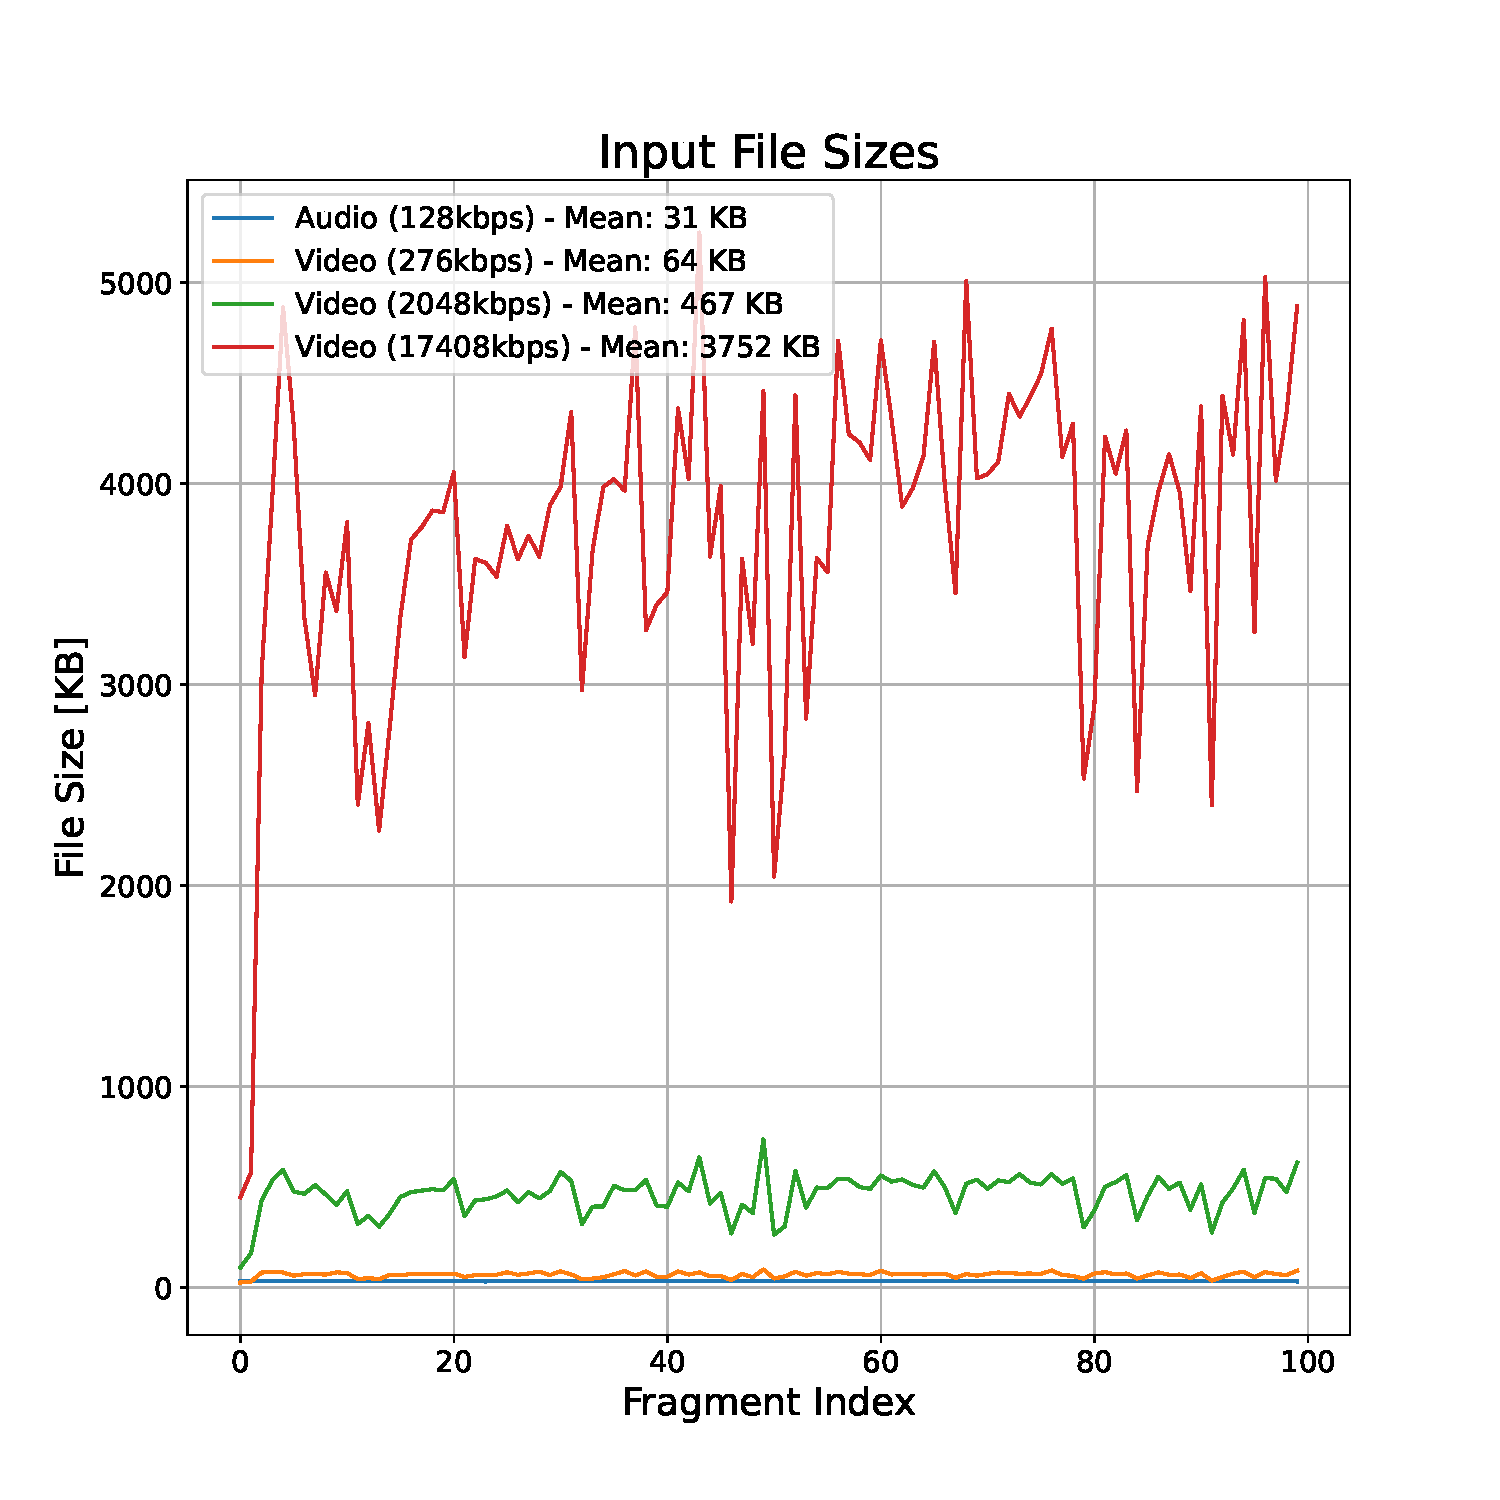
\includegraphics[width=0.75\linewidth]{plots/input-sizes.pdf}
    \caption{Input File Sizes}
    \label{fig:file-size}
\end{figure}

\subsection{Signing Duration}

In this benchmark I measured how long the entire signing function runs for to sign a live stream with up to 100 fragments. For this benchmark I loop through all available representations then for each signing method I iterate from 1 to 100 and sign the live stream at each index in accordance to the method. For the Rolling Hash signing this means that only the current fragments of that index is being signed. For the case of the optimized Merkle Tree approach I provide the signing function with the paths too all fragments to to the current index, but only the up to window size (eight) number of fragments are actually signed and for the original Merkle Tree every single fragment is being signed.

The lower the time it takes to sign the newly created fragments the less the impact on the streaming latency is, lower is better.

The time measuring can be described with the pseudo code from \Cref{alg:time-measure}. Essentially, I take a timestamp right before signing the fragments and right after the signing I take a second timestamp and the difference between the two timestamps is the time it took to sign the fragments. Then I save this value in a data structure in relation to the fragment index and representation the fragment belongs to.

\begin{algorithm}[H]
    \begin{algorithmic}[1]
        \State $now \gets Time.now()$
        \State sign\_fragments()
        \State $time \gets Time.since(now)$        
    \end{algorithmic}
    \caption{Duration Measuring Method}
    \label{alg:time-measure}
\end{algorithm}

In total I ran this benchmark ten times and averaged all results.

\subsection{Data Upload Size Required}

For this benchmark I looked at how much data has to be published to the CDN after each fragment has been signed. I measured this by simply adding up the file sizes of all the files that were effected the signing of the current fragments, which would subsequently needed to be uploaded to the CDN. In case of Rolling Hash that is only the initialization fragment and the fragment at the current index. For the optimized Merkle Tree approach that is the initialization fragment and all fragments of the current Merkle Tree, which are up to eight fragments with my configuration and again all fragments for the original Merkle Tree signing.

Since this benchmark is merely adding up file sizes I ran this one in conjunction with the previous duration benchmark, so I don't have to sign everything multiple times for each benchmark.

In this benchmark a lower upload size equals to less overhead on the network and a better caching situation for the CDN, again lower is better.

\section{Performance Measurements\label{sec:performance}}

In this section I will present the results of the above described benchmarks and give my evaluation and observations about them.

\subsection{Signing Duration}

I have split the data plots into two comparisons. One comparing each signing method in relation to the different representations, shown in \Cref{fig:sign-dur1} and the other comparing the signing method to each other per representation, shown in \Cref{fig:sign-dur2}.

This signing procedure is added step into the creation of this live stream which is why I equate the signing duration as the impact on the latency of the live stream.

Since the original Merkle Tree signing method signs every single fragment that has been created over the course of the live stream, I expected the overall signing duration to steadily increase as the live stream gets longer. This expectation is confirmed when looking at \Cref{fig:sign-dur1-og}. The signing duration of all four representations linearly increases in proportion to the number of fragments that are being included in the signing process. It can also be deduced that the larger the input files are the stronger the duration increases. 

I will score the performance of the original Merkle Tree signing method by looking at how many fragments can be signed within one second. Since the graphs are consistently linear, I will measure this score by taking the signing duration of the 100th fragment and extrapolating its signing duration to one second.

The audio representation has the lowest signing duration of all, which is expected since it has also has the lowest input file sizes with an average of \texttt{31 kilobyte}. The score of this representation is \texttt{528} fragments, which can be signing within one second. The next fastest signing duration is by the low video representations with an average file size of \texttt{64 kilobyte}. The score of this representation is \texttt{344} fragments. The mid video representation has the second slowest signing duration with average file sizes of \texttt{467 kilobyte} with a score of \texttt{82} fragment. The slowest signing duration is expectedly measured on the high video representation with average file sizes of \texttt{3,752 kilobyte} and a score of only \texttt{13} fragments.

The optimized Merkle Tree signing method uses essentially the same concepts of the original equivalent but with the added constraint that eight fragments are grouped into separate Merkle Trees. The expectations of this method is that the signing duration will look very similar for each individual Merkle Tree but reset every eight fragments. The plot in \Cref{fig:sign-dur1-opt} confirm this expectation.

The plot perfectly shows the sawtooth-signal-like graph of this approach. It starts with a low signing duration then it increases linearly like the original method and then peaks at every eighth fragment before it resets back down to the low duration. The important metric of this approach is the peak signing duration, by which I will score the individual representations.

The order slowest to fastest is the same as before. The audio representation is the fastest with a minimum signing duration around \texttt{8} milliseconds and a peak of \texttt{25} milliseconds. Again followed by the low video representation with a minimum duration of about \texttt{8} milliseconds and a peak of roughly \texttt{35} milliseconds. The next slowest is the mid video representation with the low point signing duration being on average \texttt{10} milliseconds and a maximum of around \texttt{100} milliseconds. The slowest is again the high video representation with minimum signing duration about \texttt{100} milliseconds and peaks up to \texttt{700} milliseconds.

Look at the plot of the Rolling Hash signing method in \Cref{fig:sign-dur1-rh} is clear that this is fast method overall by a good margin. Since this approach only every signs the current fragment, the signing duration directly correlates to the input file size. The three lowest representation have near constant signing duration. The audio presentation has an average of \texttt{10.5} milliseconds. The video low and mid video representations have average signing duration of \texttt{11.8} and \texttt{21.3} milliseconds, respectively. The high video representation fluctuates a lot more than the other representations but the majority of the time it remains in roughly the same interval between \texttt{80} and \texttt{100} milliseconds with an overall average of \texttt{86.5} milliseconds. When looking at the plots of \Cref{fig:sign-dur1-rh} and \Cref{fig:file-size} side by side, it is very obvious that these results are expected. The files sizes for the lower representations line up the with stability of the signing duration and the fluctuation of the higher representations equally line up with the signing durations.

\begin{figure}
    \centering
    \subfloat[Original Merkle Tree]{
        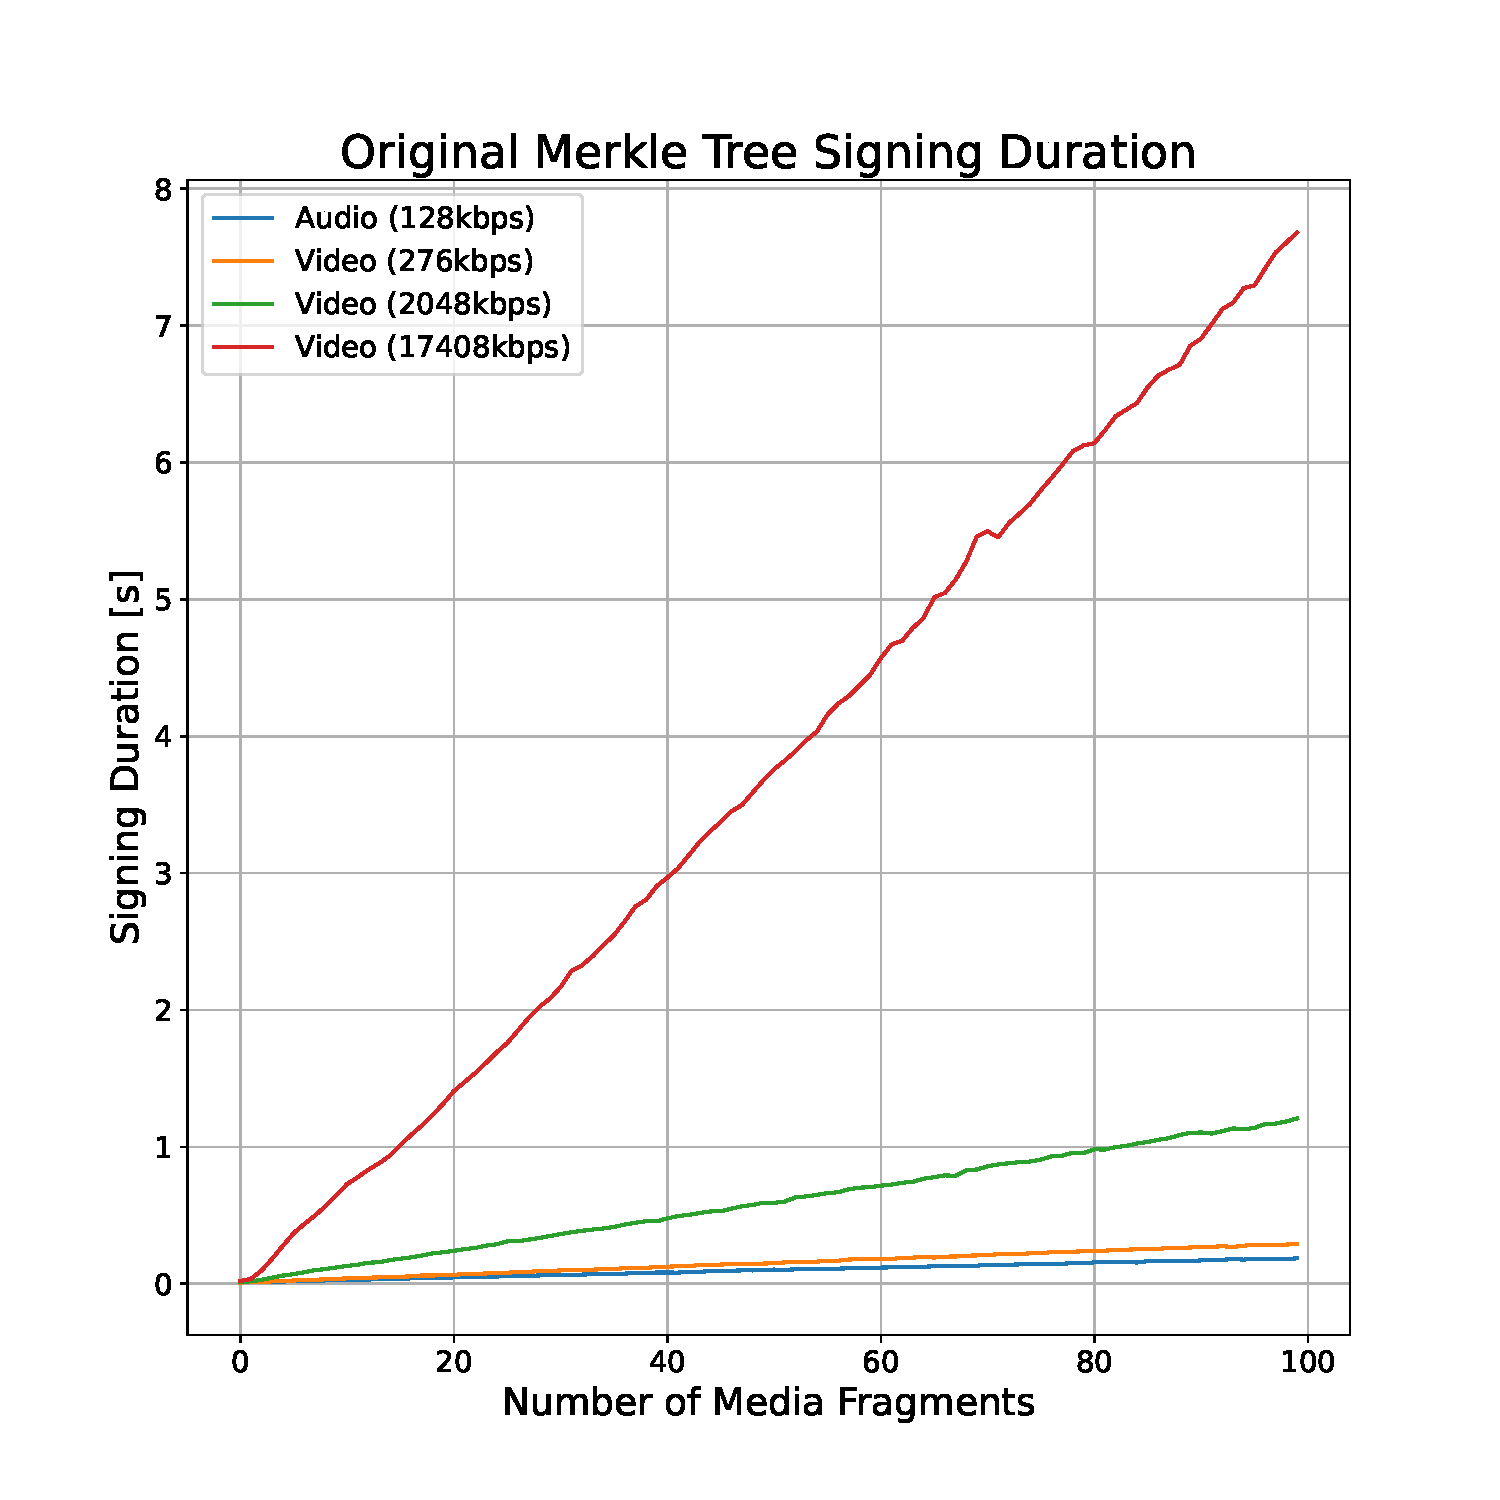
\includegraphics[width=0.49\linewidth]{plots/time-original-merkle-tree.pdf}
        \label{fig:sign-dur1-og}
    }
    \subfloat[Optimized Merkle Tree]{
        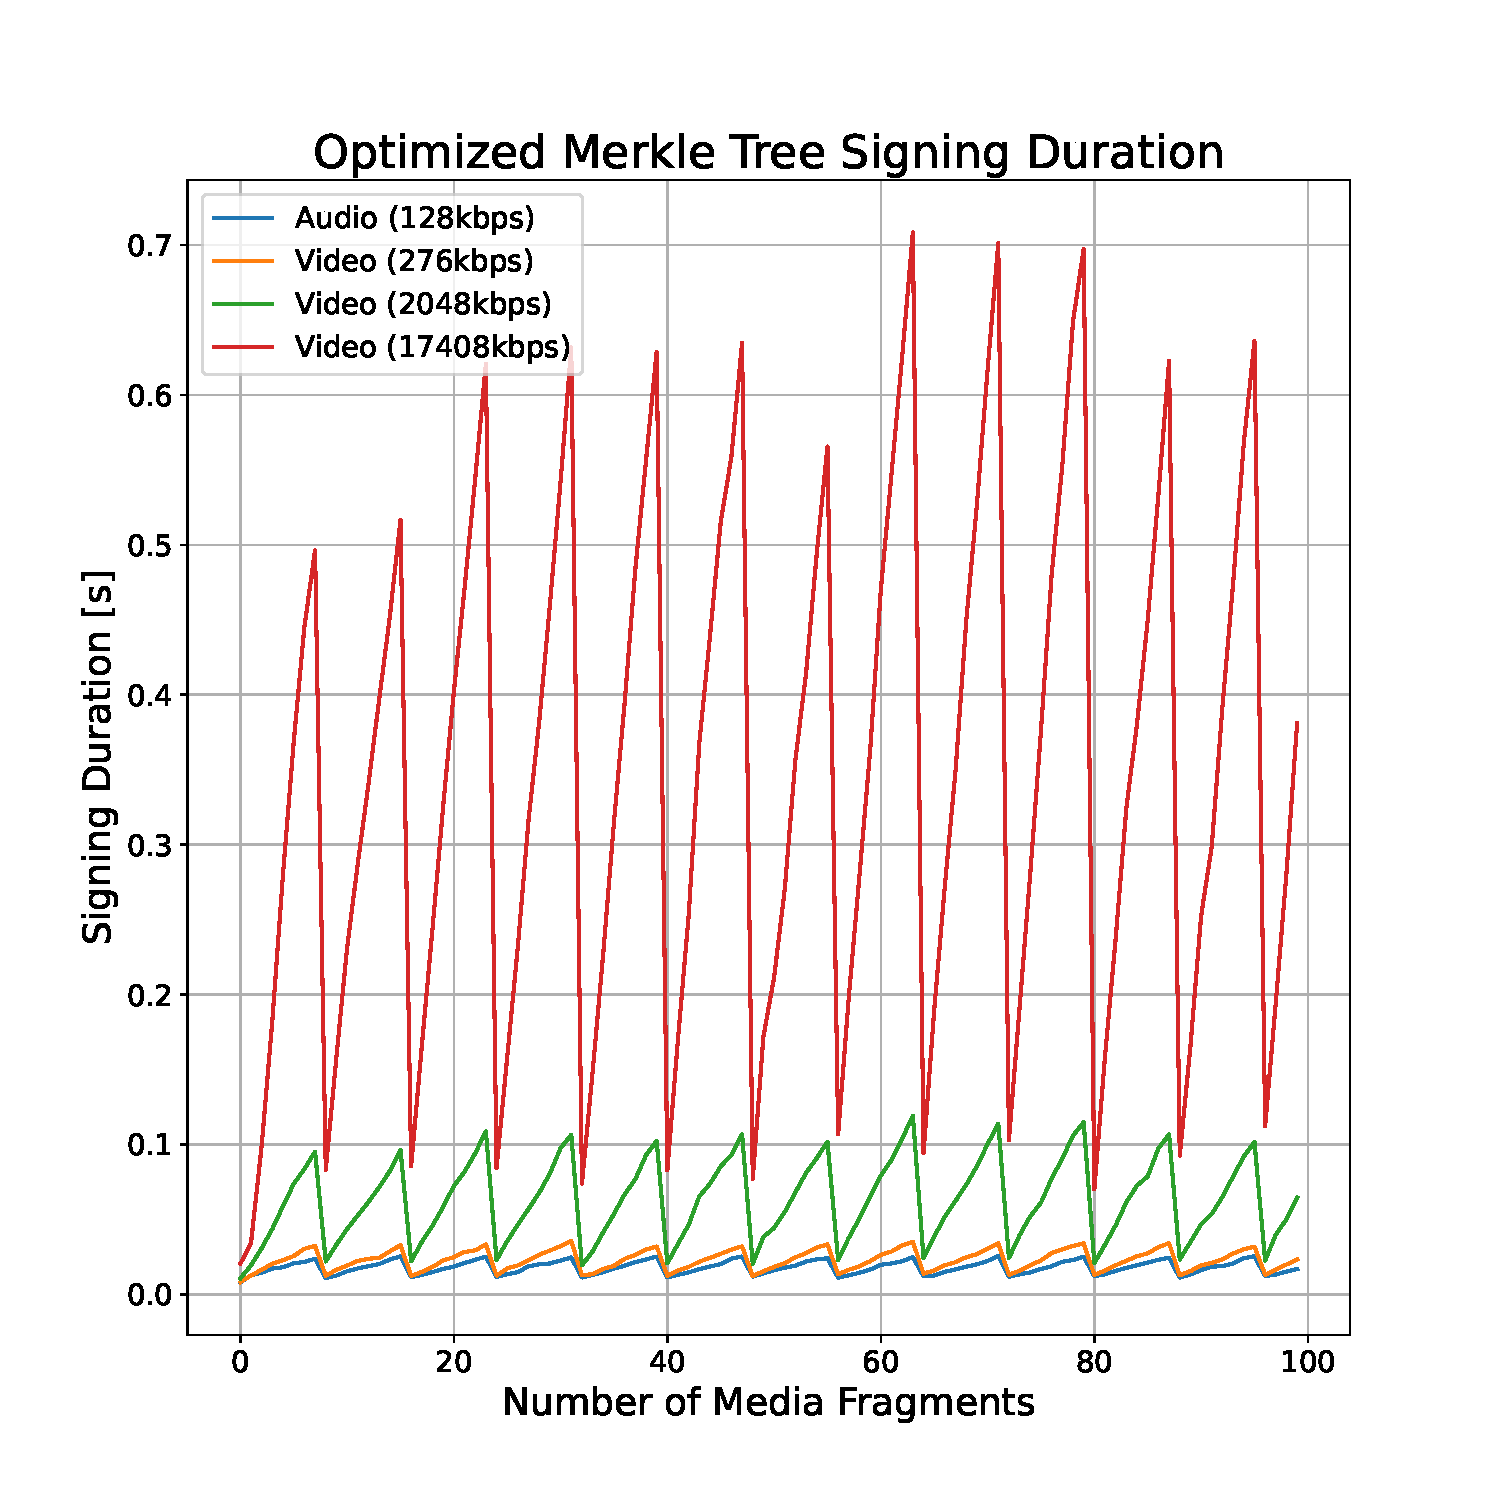
\includegraphics[width=0.49\linewidth]{plots/time-optimized-merkle-tree.pdf}
        \label{fig:sign-dur1-opt}
    } \\
    \subfloat[Rolling Hash]{
        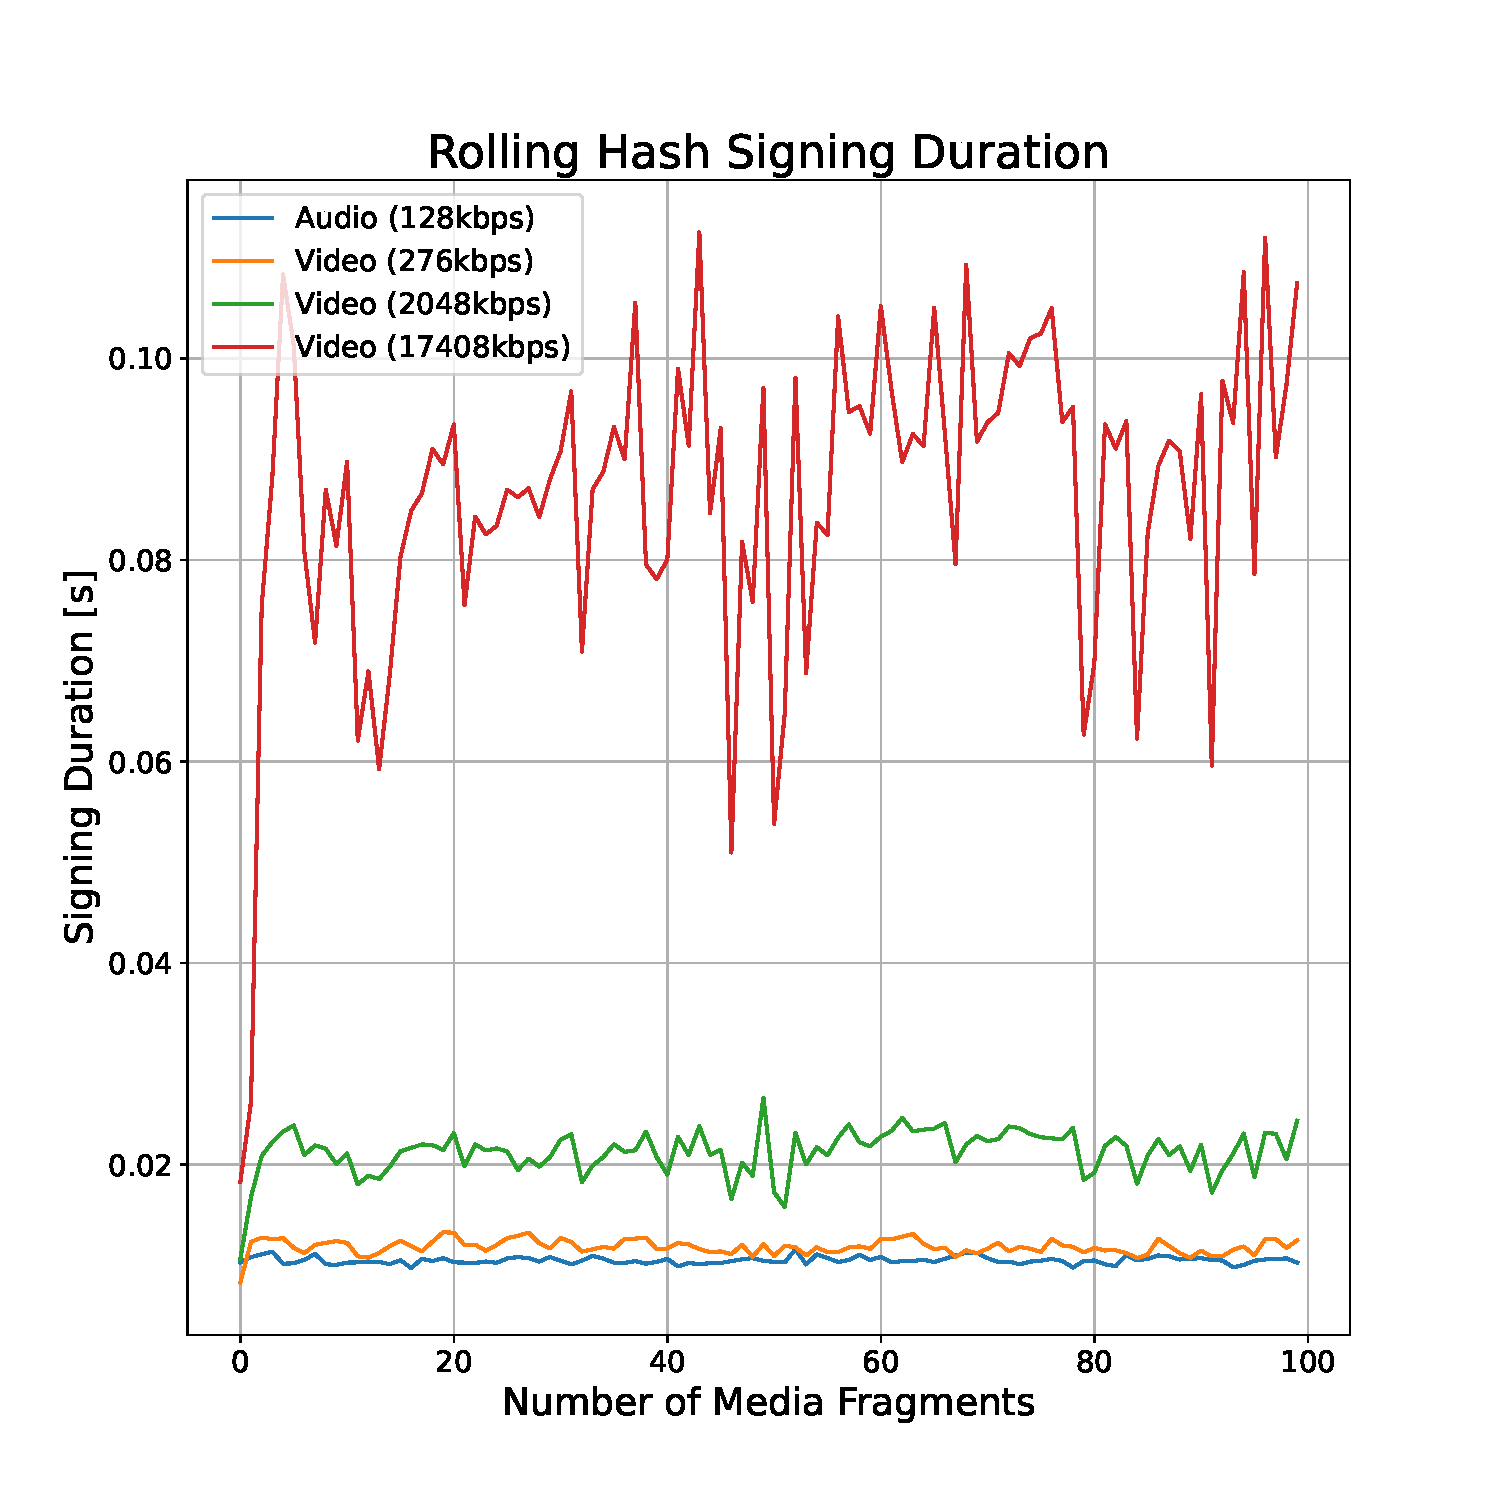
\includegraphics[width=0.49\linewidth]{plots/time-rolling-hash.pdf}
        \label{fig:sign-dur1-rh}
    }
    \caption{Signing Duration Results}
    \label{fig:sign-dur1}
\end{figure}

Now looking at the comparison of the signing methods to each other in \Cref{fig:sign-dur2}, it gets directly apparent that the signing methods all perform essentially the same in regards to what representation is being signed. However, these plots show very well that the original signing method is by a large margin the lowest signing method, with the optimized Merkle Tree signing method being much more competitive with the Rolling Hash method but the Rolling Hash method is still the best without a doubt.

\begin{figure}
    \centering
    \subfloat[Audio (128kbps)]{
        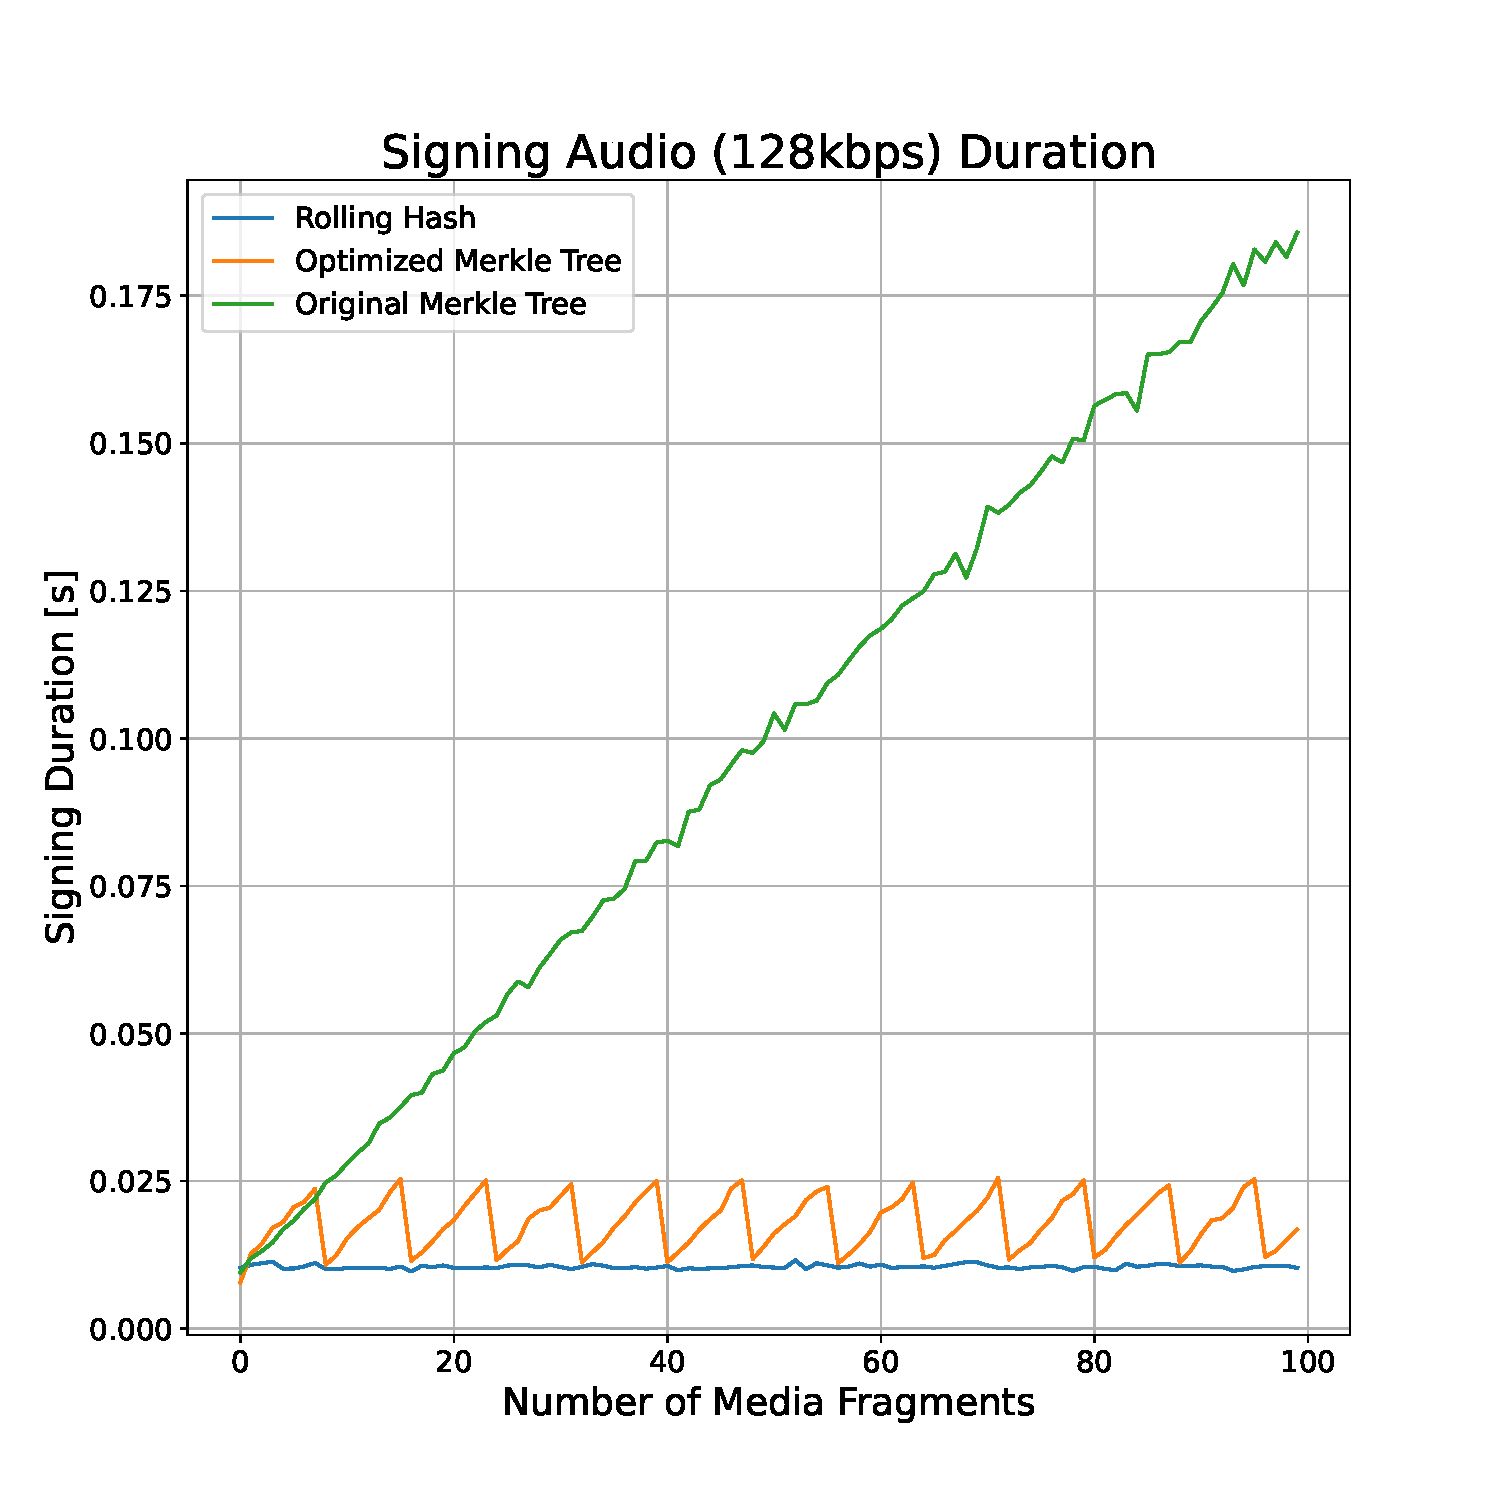
\includegraphics[width=0.49\linewidth]{plots/compare-time-Audio-(128kbps).pdf}
        \label{fig:sign-dur2-audio}
    }
    \subfloat[Video (276kbps)]{
        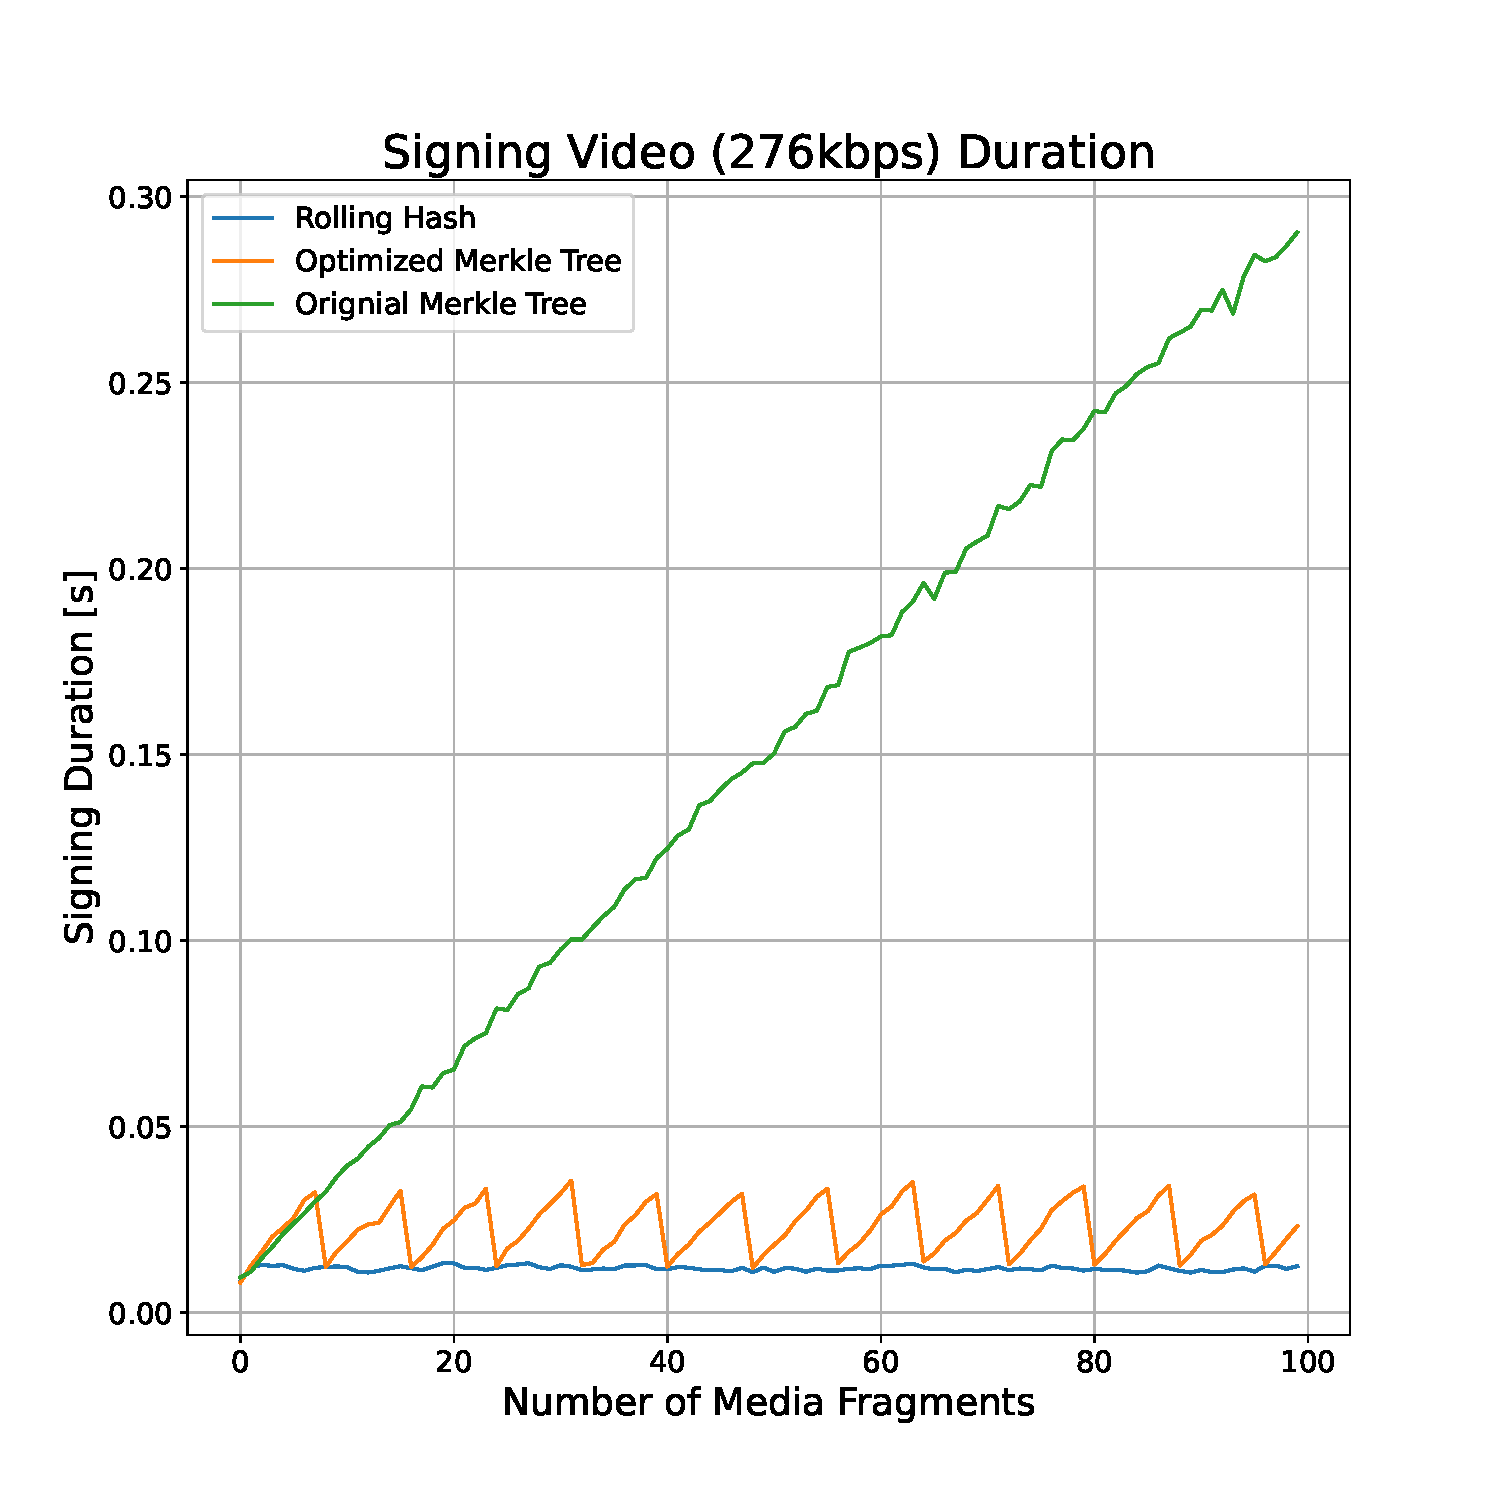
\includegraphics[width=0.49\linewidth]{plots/compare-time-Video-(276kbps).pdf}
        \label{fig:sign-dur2-video1}
    } \\
    \subfloat[Video (2,048kbps)]{
        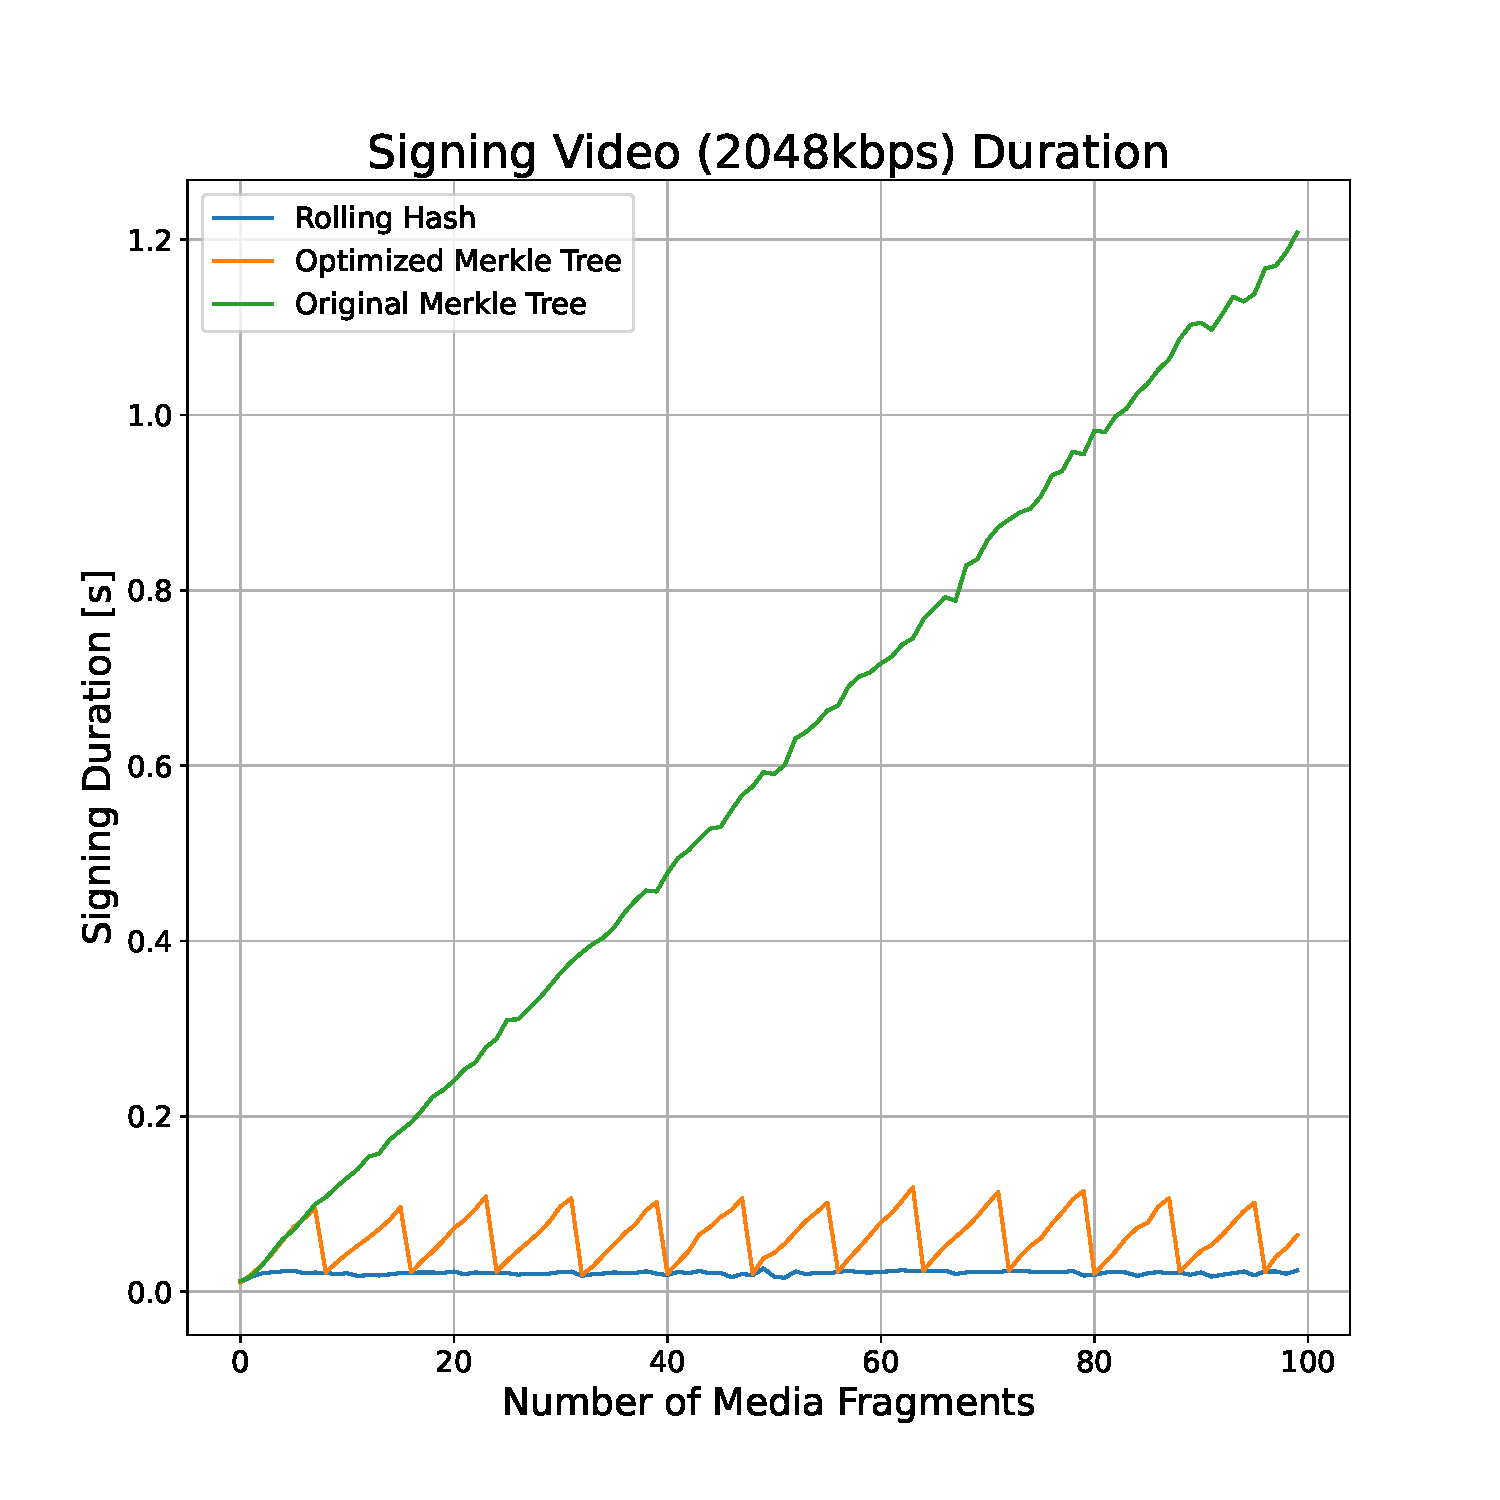
\includegraphics[width=0.49\linewidth]{plots/compare-time-Video-(2048kbps).pdf}
        \label{fig:sign-dur2-video2}
    }
    \subfloat[Video (17,408kbps)]{
        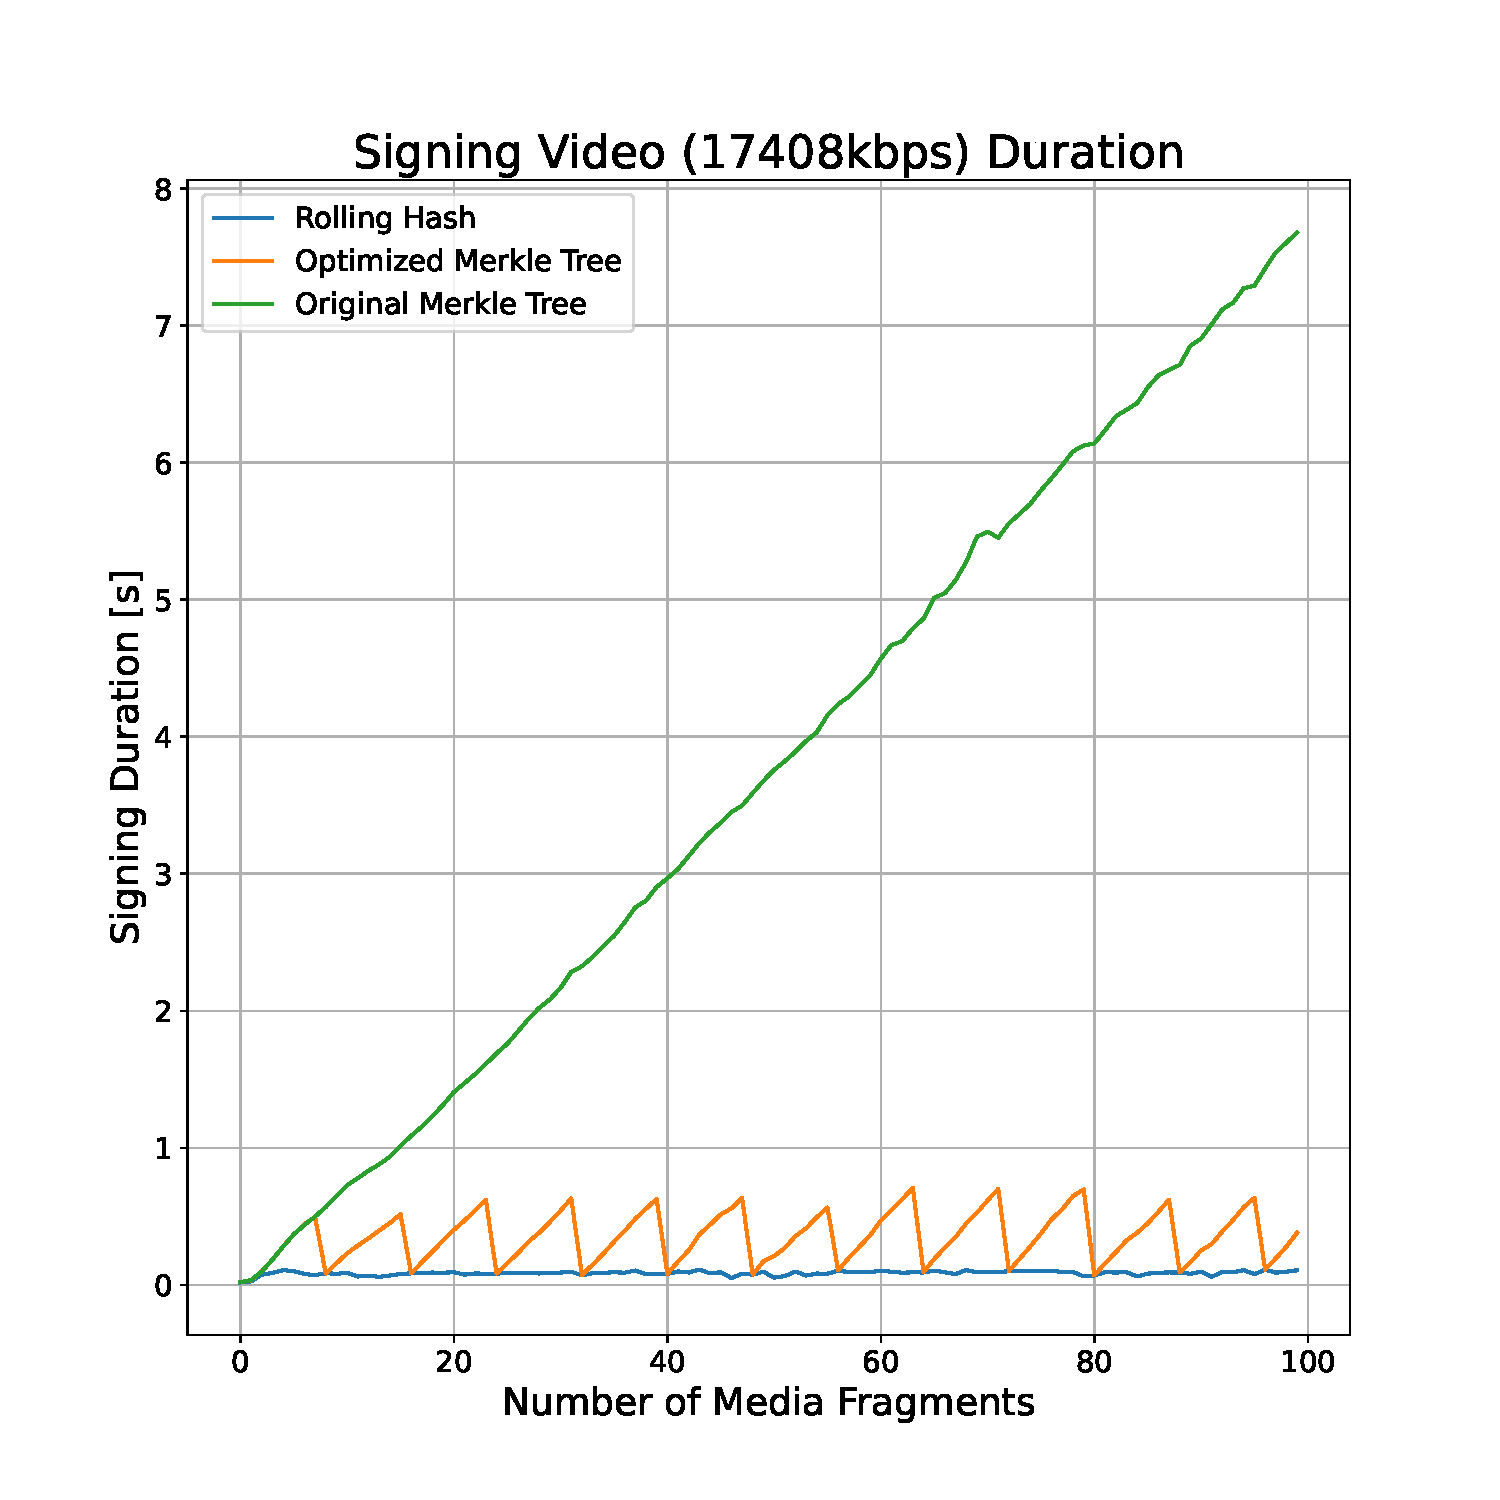
\includegraphics[width=0.49\linewidth]{plots/compare-time-Video-(17408kbps).pdf}
        \label{fig:sign-dur2-video3}
    }
    \caption{Signing Duration Results}
    \label{fig:sign-dur2}
\end{figure}

\subsection{Data Upload Size Required}

For this benchmark I have split the data plots into the same comparisons as before: comparing each signing method in relation to the different representations are shown in \Cref{fig:upload1} and the signing methods compared to each other per representation are shown in \Cref{fig:upload2}.

In essence, the results of the required data upload size is exactly the same as the signing duration benchmark. The original Merkle Tree method requires by far the most data upload, of which the majority is entirely redundant, because every time a new fragment is being signed, every single prior fragment is being signed as well and subsequently they are have to be published anew to the CDN to have the most up-to-date data available. As before it also shows a linear increase as the number of fragment rises. All the representations have an gradient of slightly more then the average file size per fragment, as shown in \Cref{fig:file-size}. The reason by this is that with every new fragment everything from before has to be uploaded again, as already mentioned and the gradient is a little more because the added C2PA data is now included in the files. These results are shown in \Cref{fig:upload1-og}.

The same goes for the optimized Merkle Tree signing approach, shown in \Cref{fig:upload1-opt}. Again a sawtooth-signal-like graph can be observed which resets every eighth fragment. In all cases the needed upload is considerably lower than compared to the original method.

Lastly, the Rolling Hash results are equally the same, as seen in \Cref{fig:upload1-rh}. The three lower representations again have a near constant value and the highest fluctuates slightly but overall still significantly lower than the other two methods.

\begin{figure}
    \centering
    \subfloat[Original Merkle Tree]{
        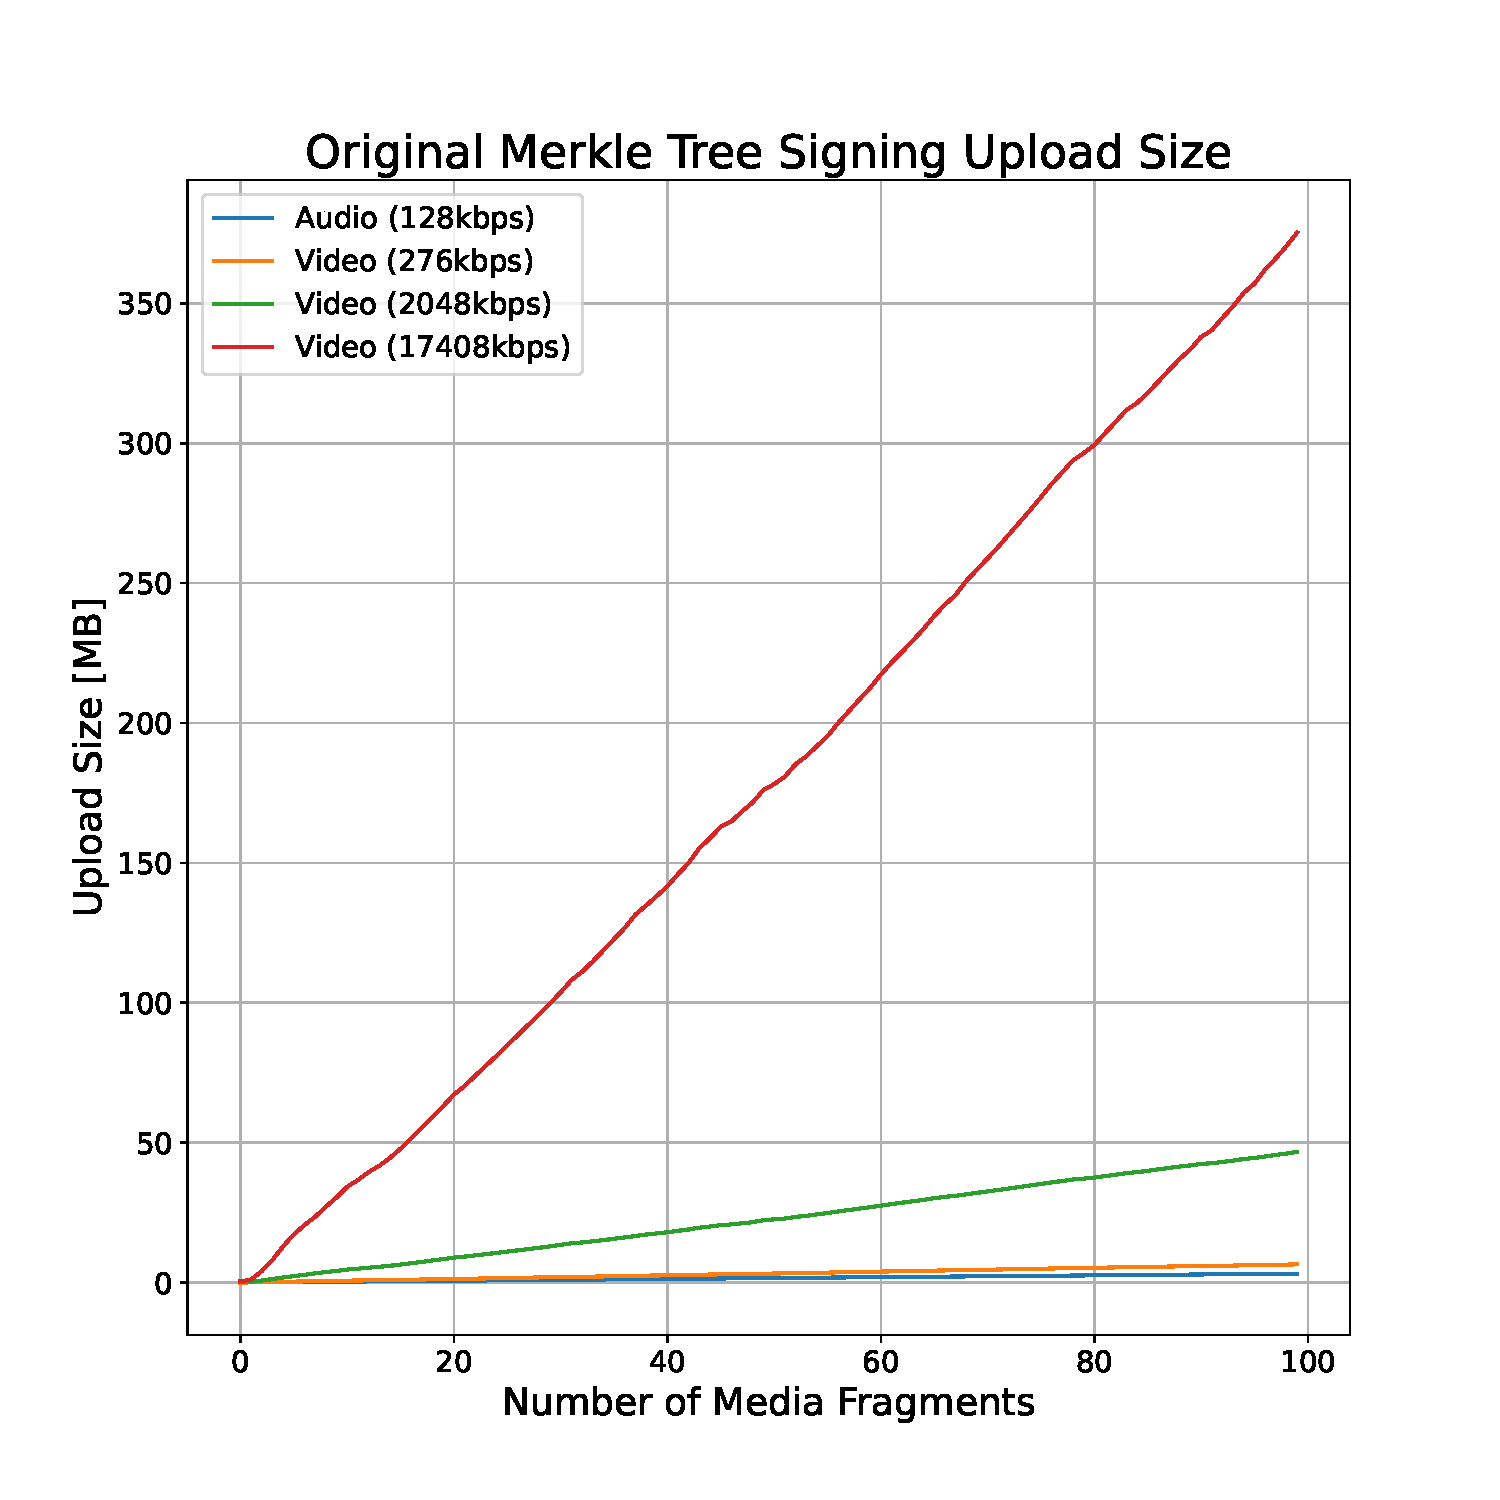
\includegraphics[width=0.49\linewidth]{plots/upload-original-merkle-tree.pdf}
        \label{fig:upload1-og}
    }
    \subfloat[Optimized Merkle Tree]{
        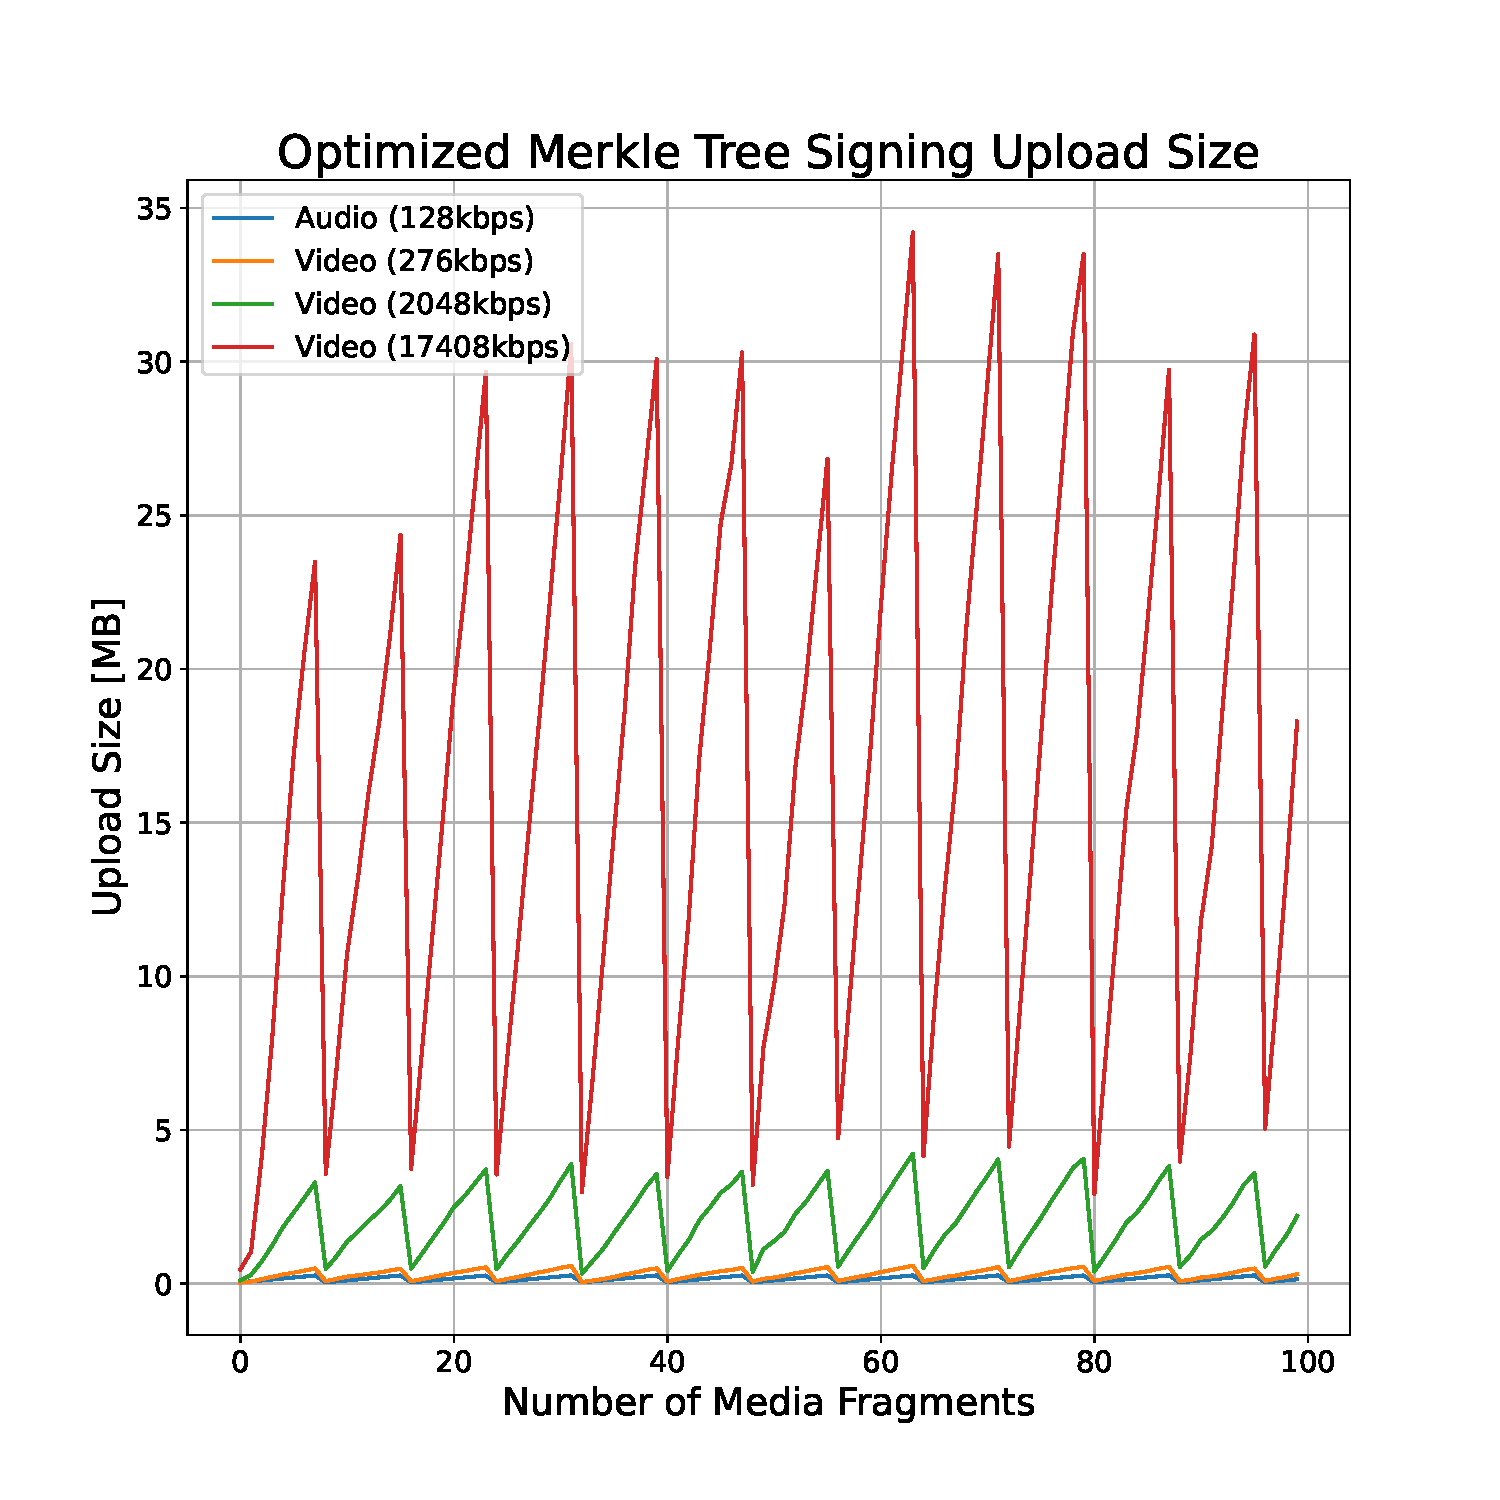
\includegraphics[width=0.49\linewidth]{plots/upload-optimized-merkle-tree.pdf}
        \label{fig:upload1-opt}
    } \\
    \subfloat[Rolling Hash]{
        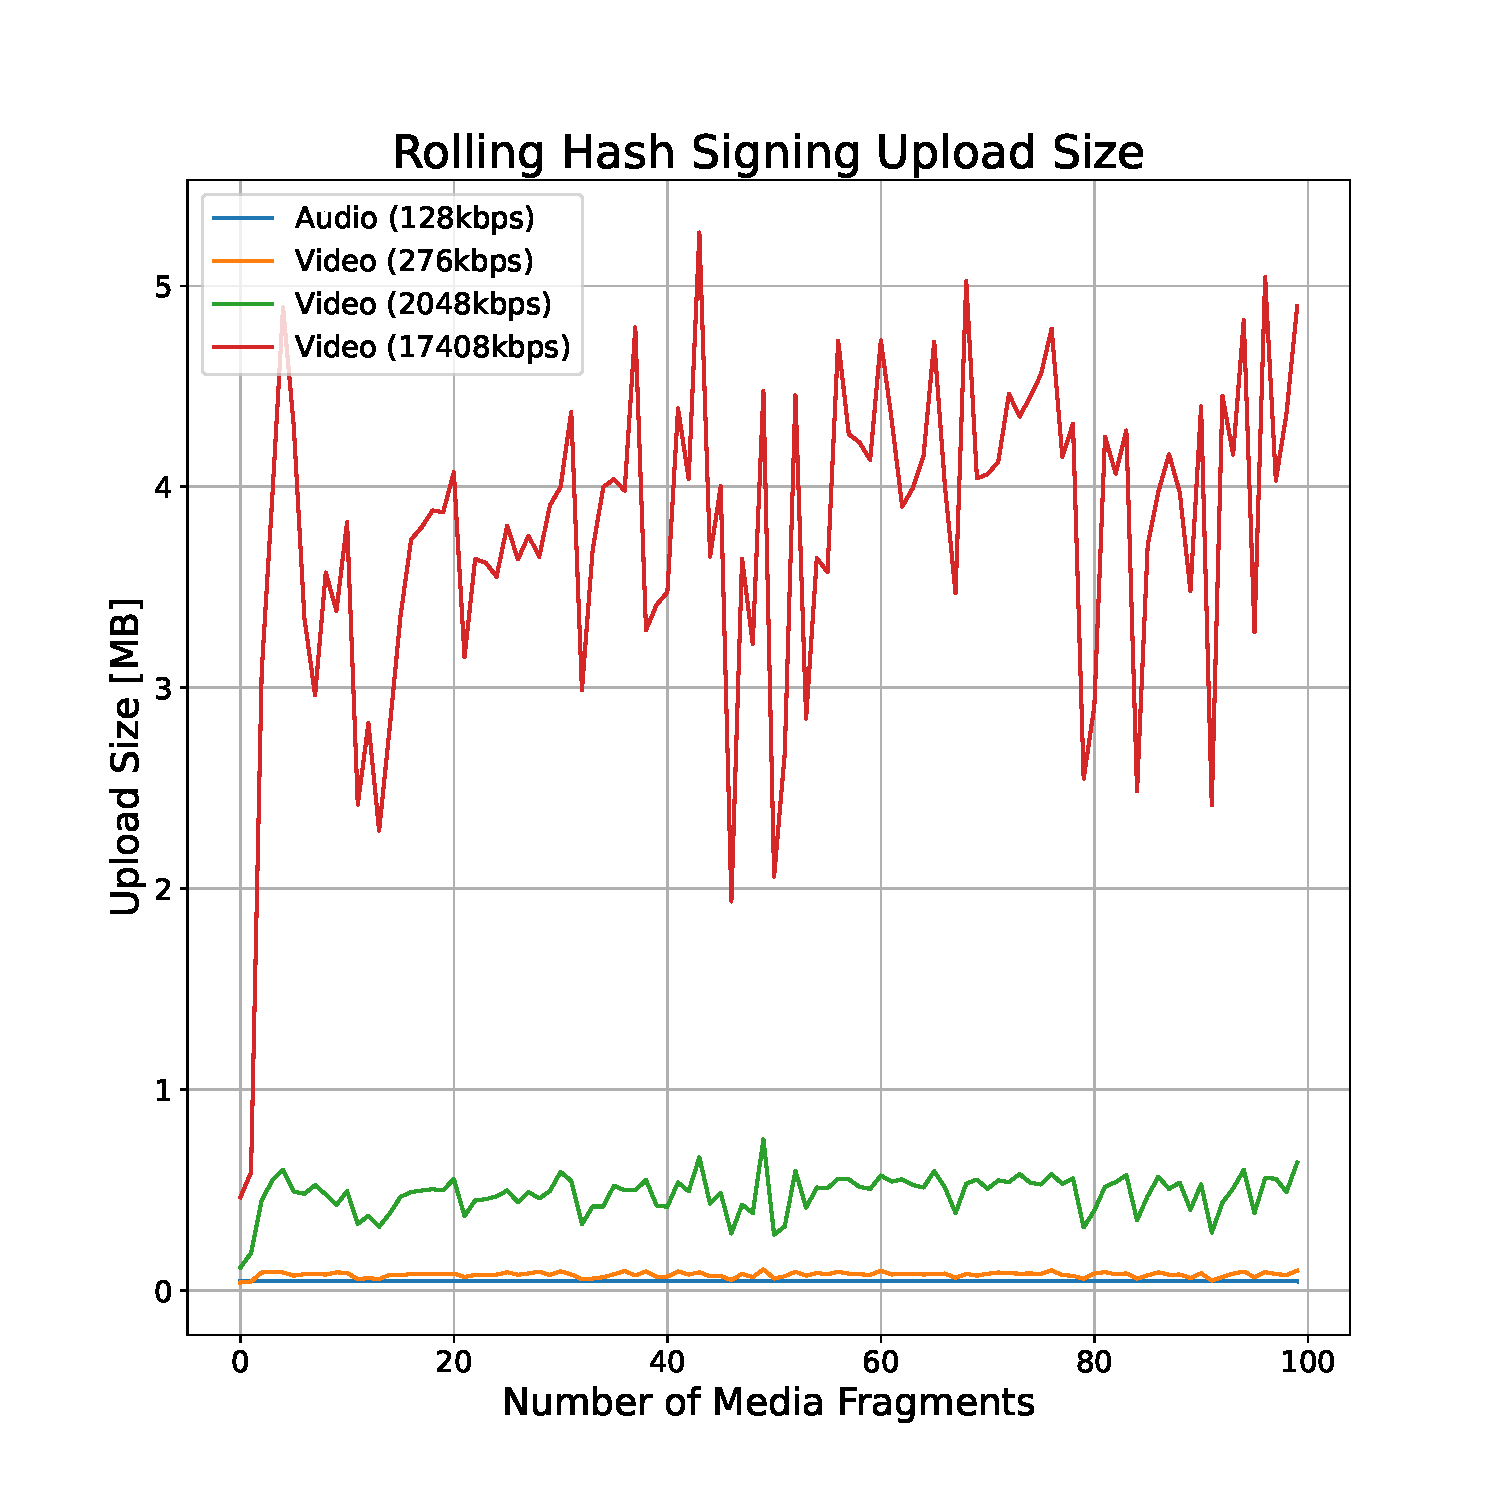
\includegraphics[width=0.49\linewidth]{plots/upload-rolling-hash.pdf}
        \label{fig:upload1-rh}
    }
    \caption{Upload Size Results}
    \label{fig:upload1}
\end{figure}

\begin{figure}
    \centering
    \subfloat[Audio (128kbps)]{
        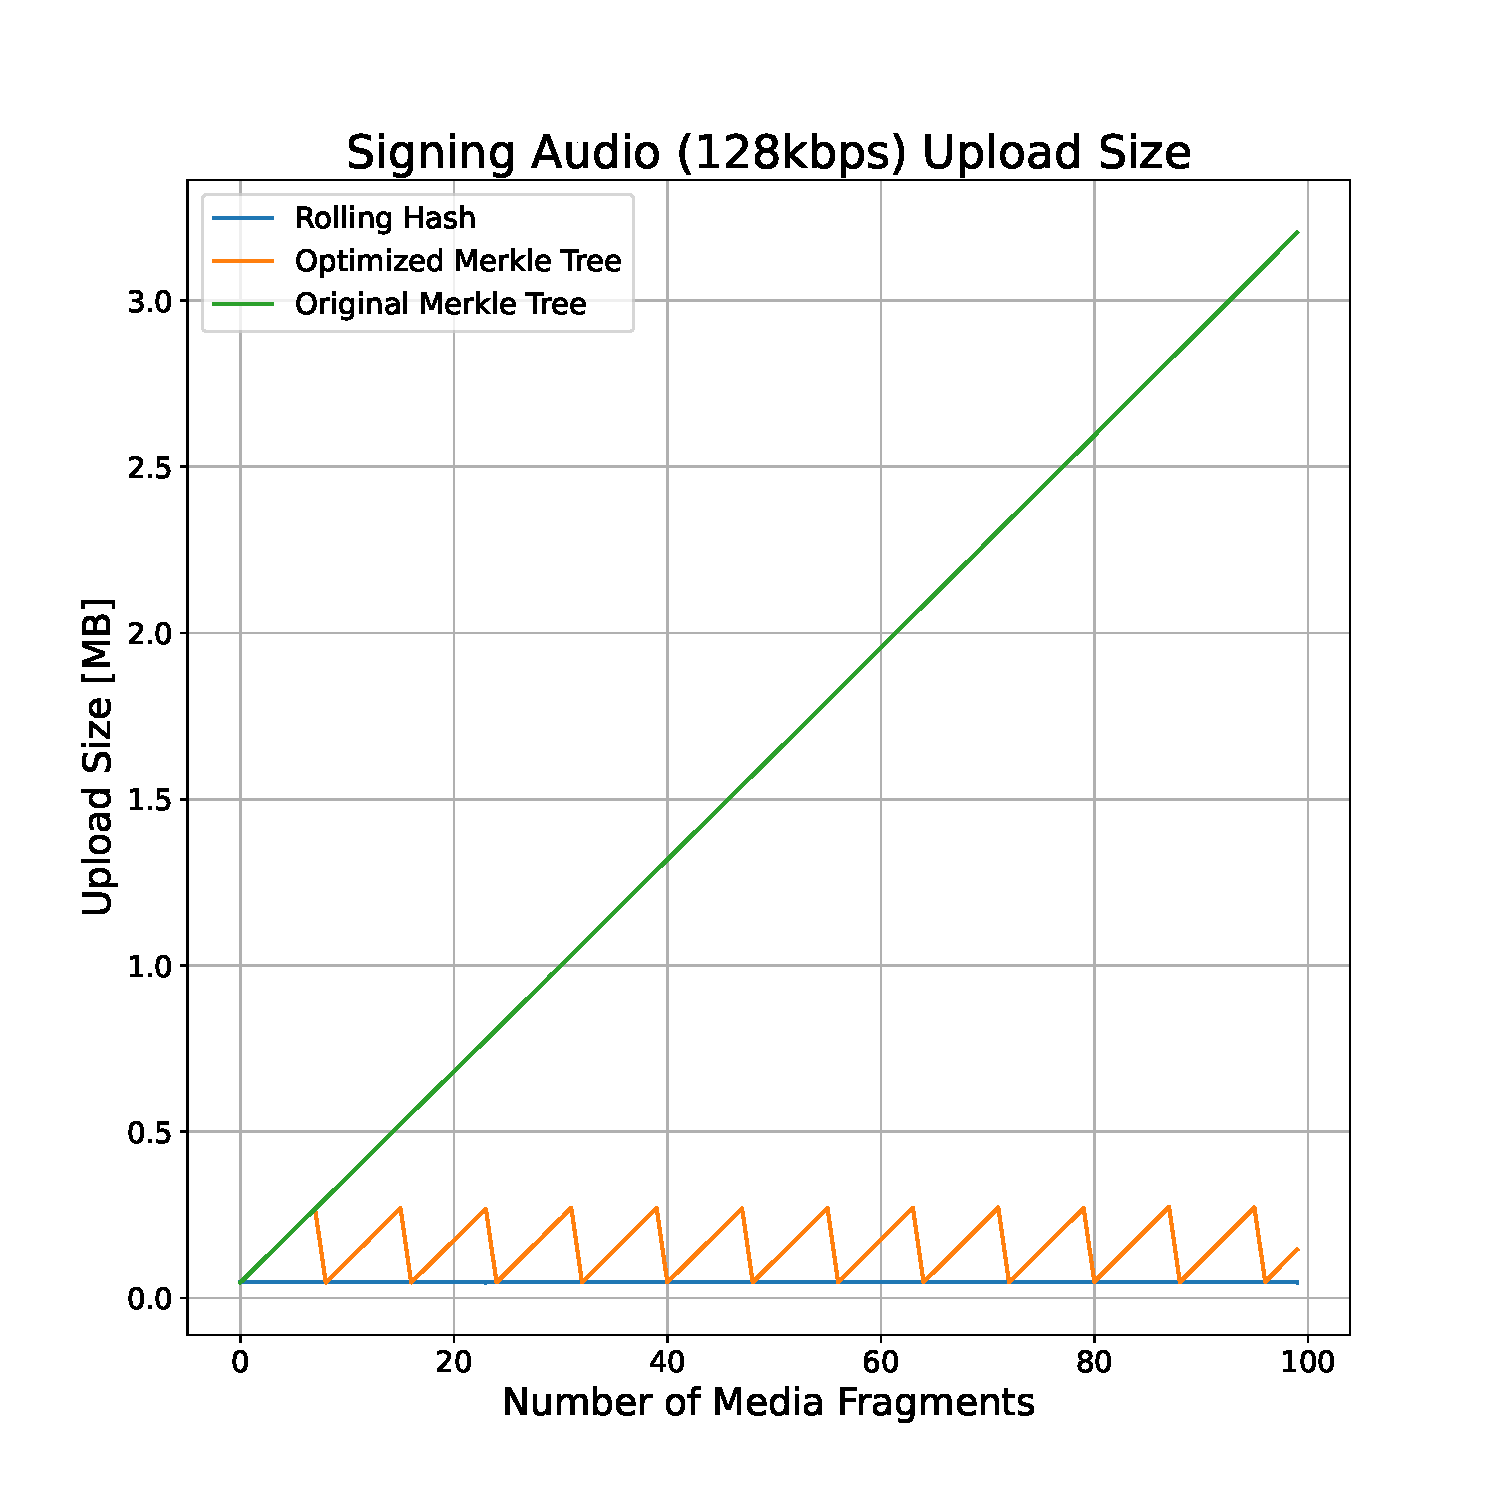
\includegraphics[width=0.49\linewidth]{plots/compare-upload-Audio-(128kbps).pdf}
        \label{fig:upload2-audio}
    }
    \subfloat[Video (276kbps)]{
        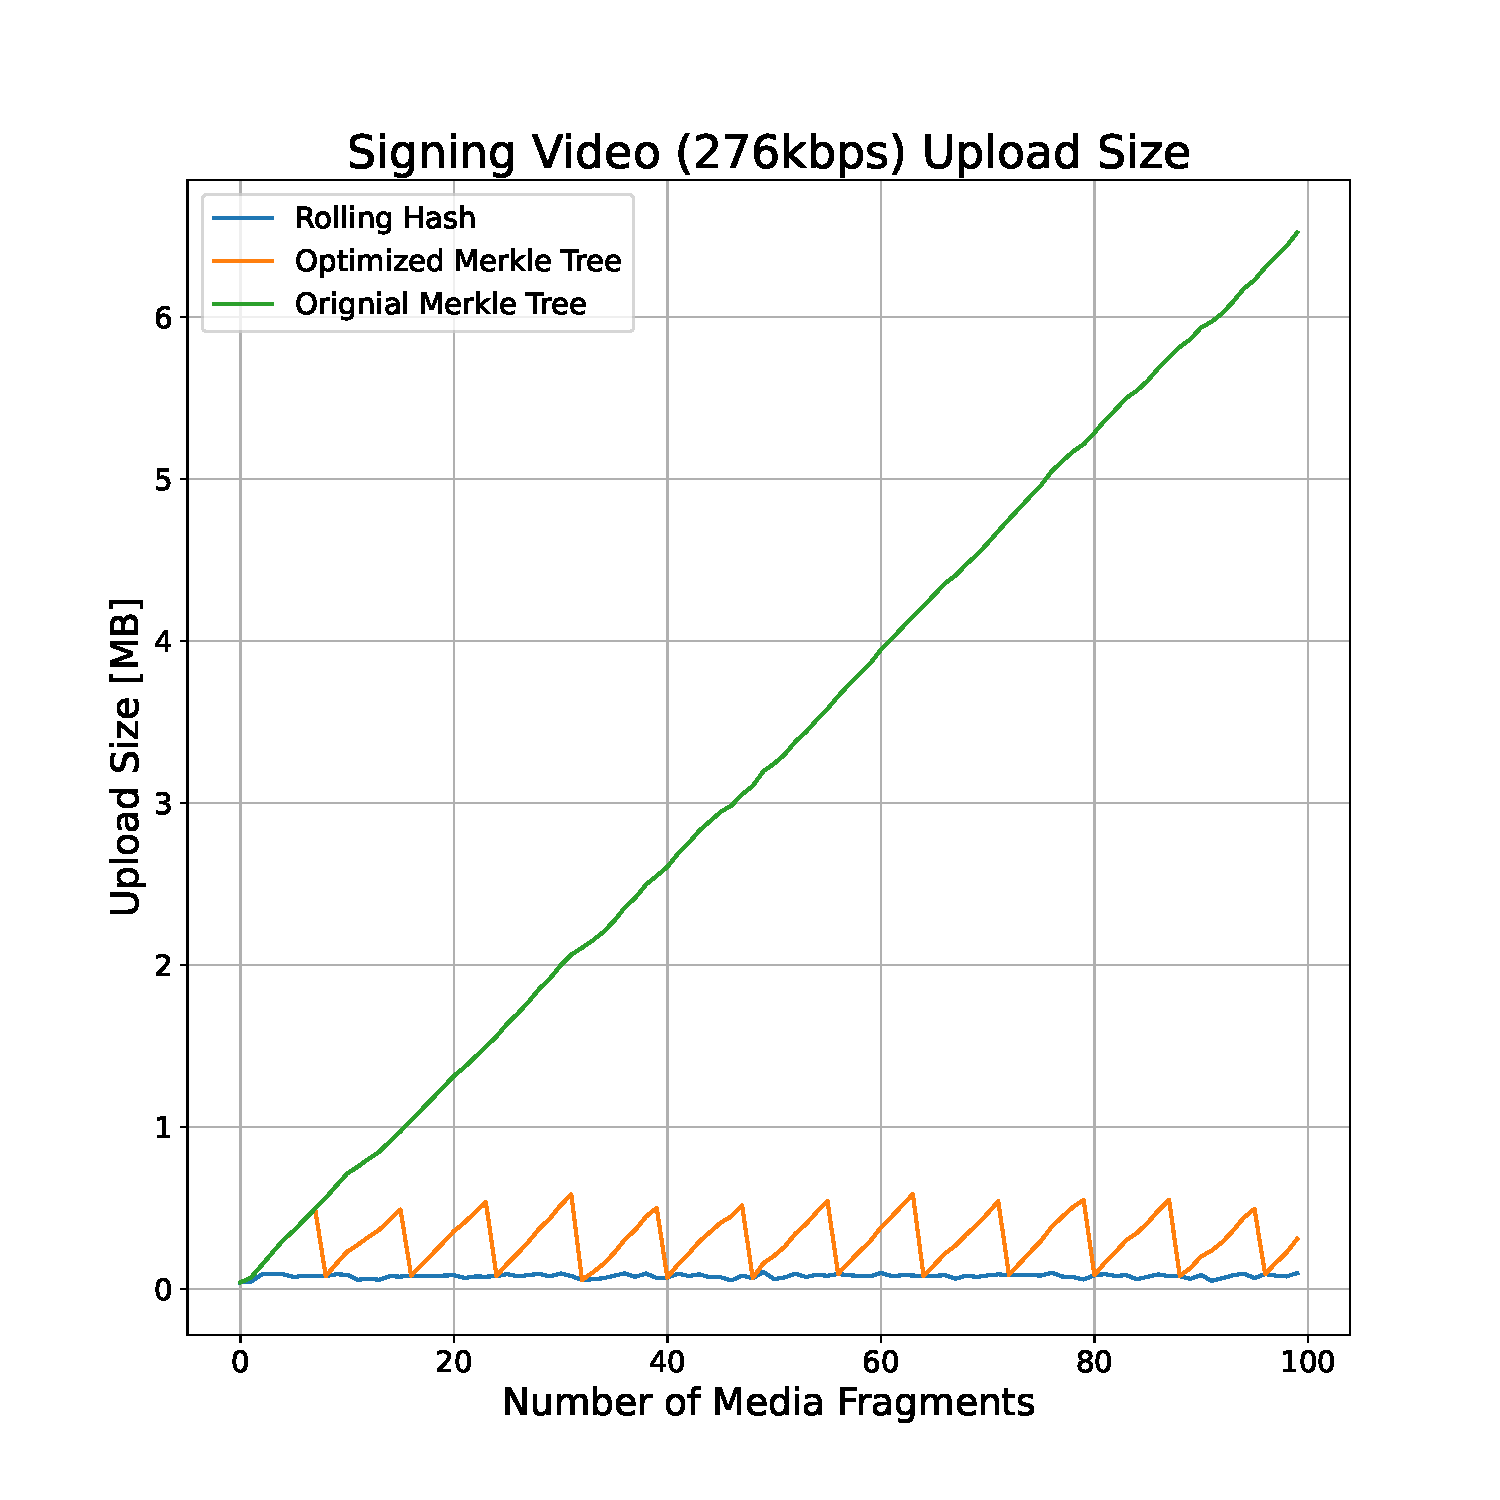
\includegraphics[width=0.49\linewidth]{plots/compare-upload-Video-(276kbps).pdf}
        \label{fig:upload2-video1}
    } \\
    \subfloat[Video (2,048kbps)]{
        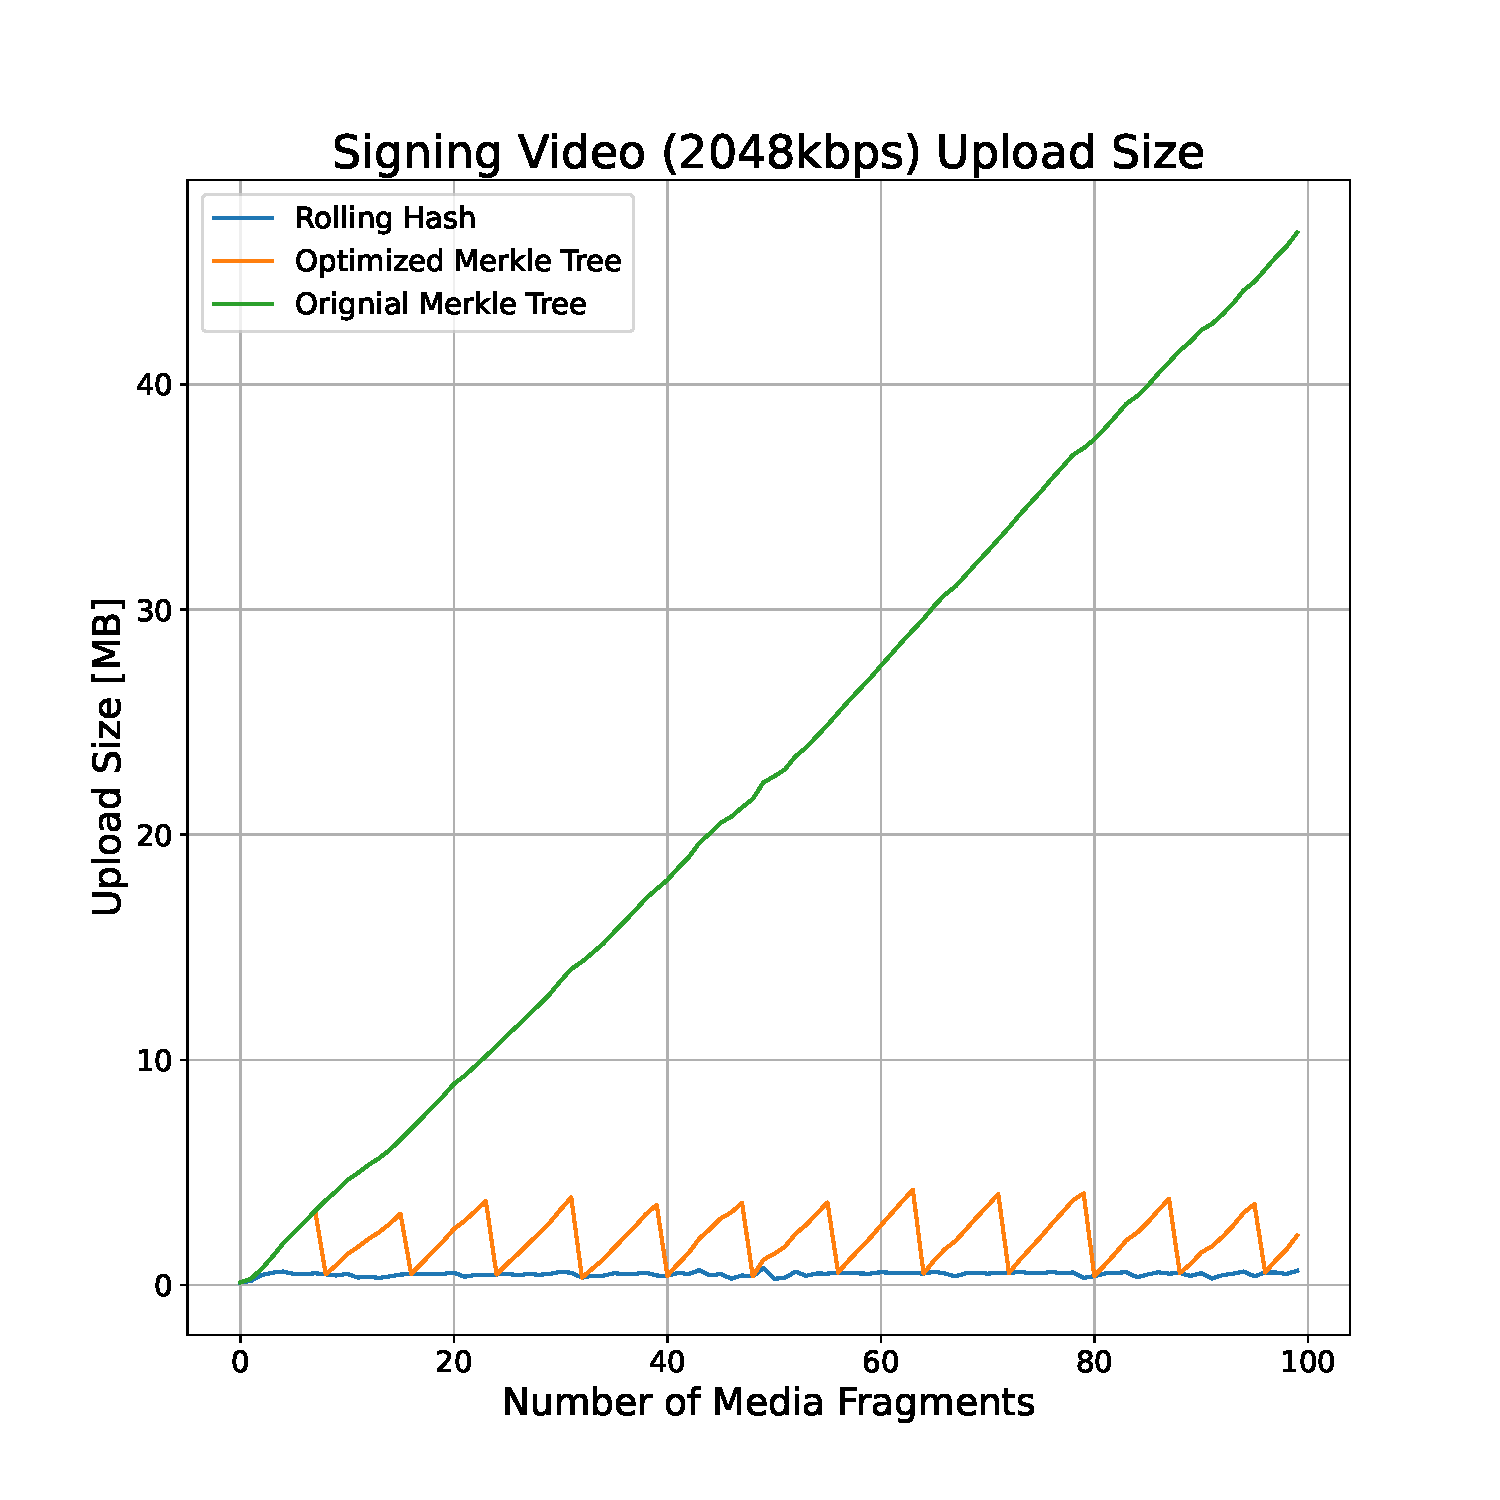
\includegraphics[width=0.49\linewidth]{plots/compare-upload-Video-(2048kbps).pdf}
        \label{fig:upload2-video2}
    }
    \subfloat[Video (17,408kbps)]{
        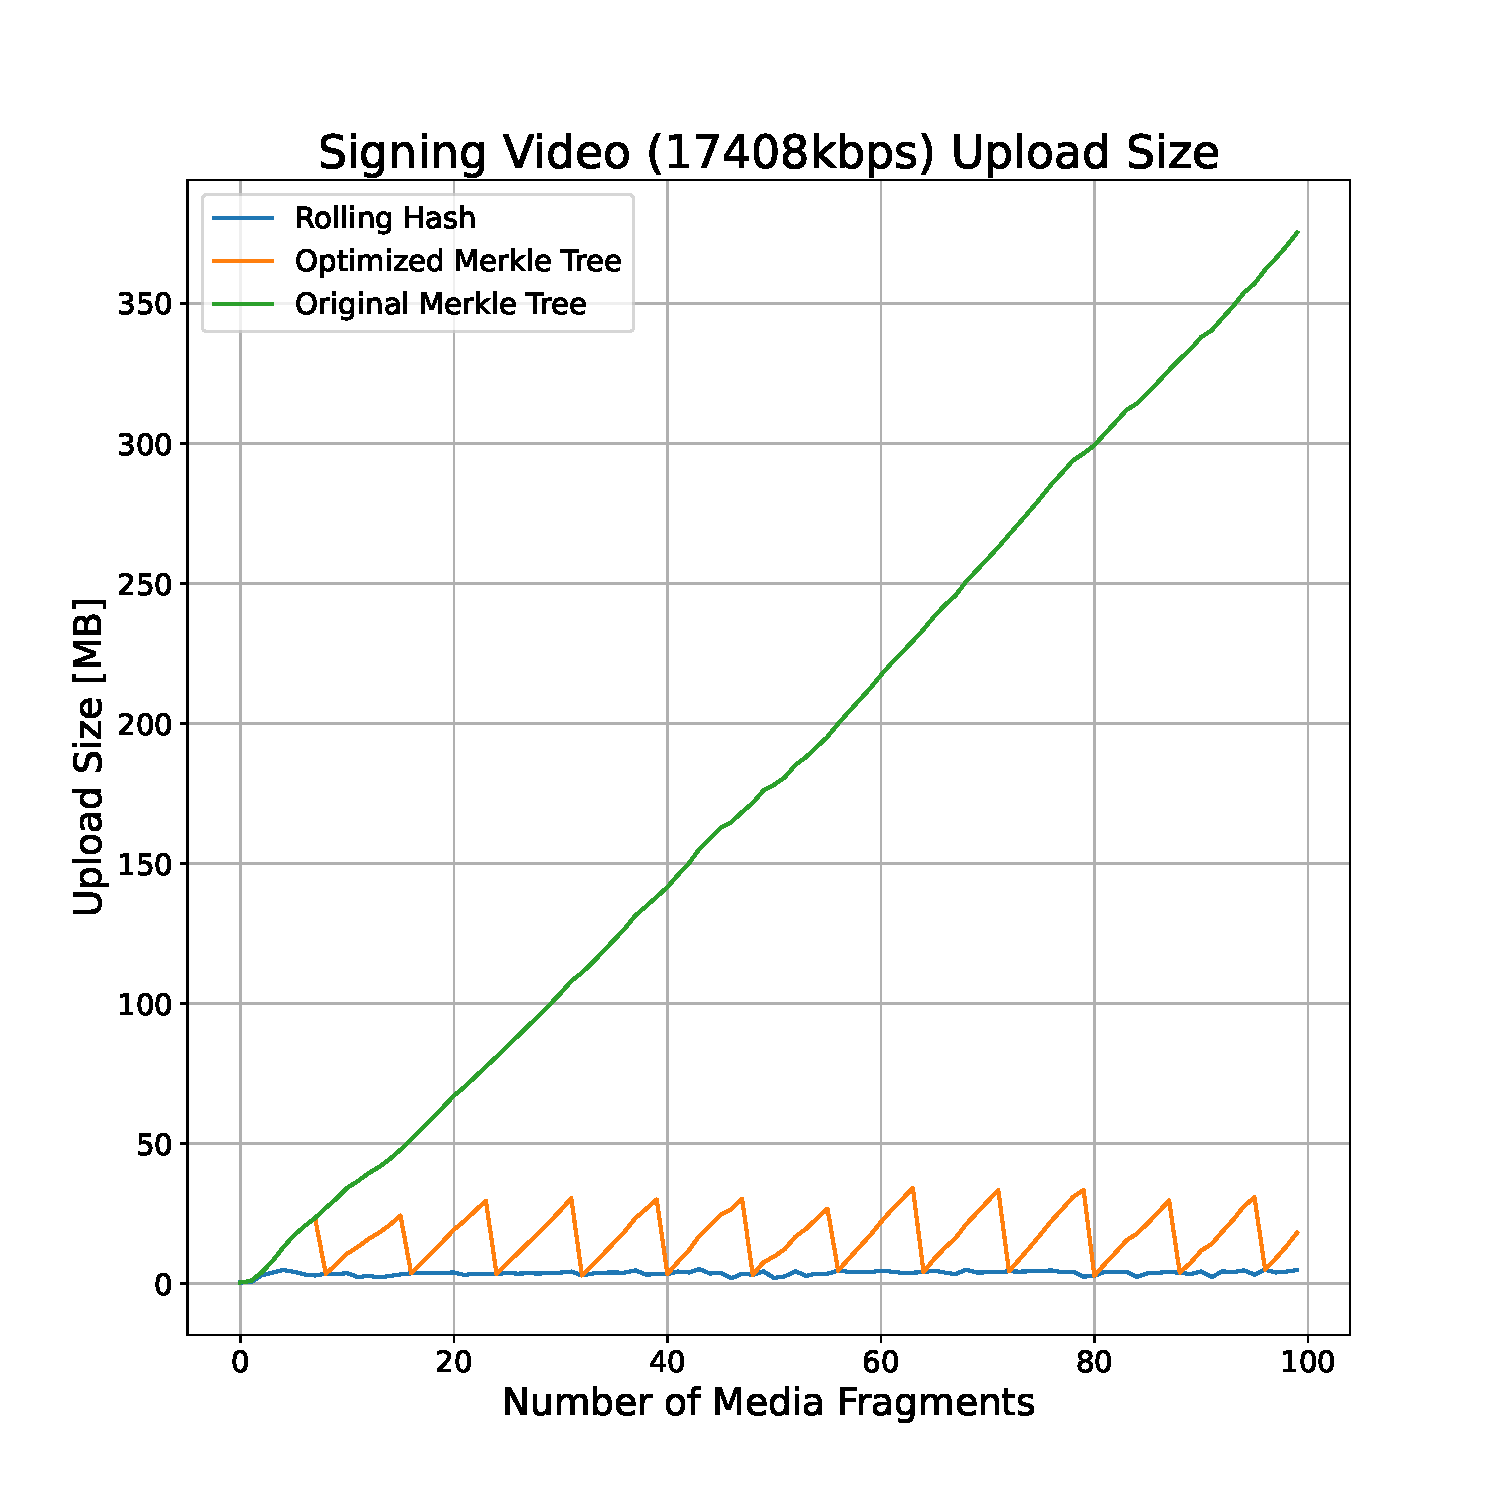
\includegraphics[width=0.49\linewidth]{plots/compare-upload-Video-(17408kbps).pdf}
        \label{fig:upload2-video3}
    }
    \caption{Upload Size Results}
    \label{fig:upload2}
\end{figure}


    \chapter{Conclusion\label{cha:chapter7}}

in Conclusion...

\section{Summary\label{sec:summary}}



\section{Dissemination\label{sec:dissemination}}



\section{Problems Encountered\label{sec:problems}}



\section{Outlook\label{sec:outlook}}

integration in to more, devices, platforms, tools, maturing the implementation, availability

connecting to MoQT, breaking everything into chunks and periodic update are the bread and butter of MoQT

% ---------------------------------------------------------------
\backmatter % no page numbering from here
    \todo[inline]{talk to your supervisor if this is needed}
    \addchap{List of Acronyms}

\begin{tabbing}
spacespacespace \= space \kill
API	    \> 	    Application Programming Interface	 \\
BMFF    \>      Base Media File Format \\
C2PA    \>      Coalition of Content Provenance and Authenticity \\
CLI     \>      Command Line Interface \\
CDN     \>      Content Delivery Network \\
CSS	    \>	    Cascading Style Sheets \\
DASH    \>      Dynamic Adaptive Streaming over HTTP \\
FOKUS	\>	    Fraunhofer Institut fuer offene Kommunikationssysteme \\
GUI	    \>	    Graphical User Interface \\
HLS     \>      HTTP Live Streaming \\
HTML	\>	    Hypertext Markup Language \\
HTTP	\>      Hypertext Transfer Protocol	 \\
IP	    \> 	    Internet Protocol	 \\
JSON	\>	    JavaScript Object Notation \\
MPD     \>      Media Presentation Description \\
URI	    \> 	    Uniform Resource Identifier	 \\
VoD     \>      Video on Demand \\
XML	    \> 	    Extensible Markup Language	 \\
\end{tabbing}
\endinput

		
		% if you want to provide a glossary with explanations of important terms put it in here

    \bibliographystyle{geralpha}
    \bibliography{./bib/manual}
    
    \addchap{Annex}

\begin{appendix}

\begin{minipage}{\linewidth}
\begin{lstlisting}[caption={Example FFmpeg Shell Script}, label=ex:shell, captionpos=b]
#!/usr/bin/env bash

# change directory to this file to  
# make it runnable from anywhere
cd "$(dirname "$0")" || exit
    
# use ENV variables to override configured defaults
OUTPUT="${OUTPUT:-http://localhost:6262/ingest/bbb/source.mpd}"
    
ffmpeg \
    -loglevel error -stats -hide_banner \
    -f lavfi -re -i testsrc=size=1280x720:rate=25 \
    -profile main \
    -pix_fmt yuv420p \
    -map 0:v:0 -s:v:0 1280x720 -b:v:0 2048000 \
-maxrate:v:0 2200000 -bufsize:v:0 3300000 \
    -f dash \
    -dash_segment_type mp4 \
    -preset medium \
    -sc_threshold 0 \
    -r 25 \
    -keyint_min 48 \
    -g 48 \
    -c:v libx264 \
    -hls_playlist 1 \
    -master_m3u8_publish_rate 1 \
    -http_persistent 1 \
    -adaptation_sets "id=0,streams=v" \
    -seg_duration 1.920 \
    -update_period 1.920 \
    -use_template 1 \
    -use_timeline 1 \
    -utc_timing_url https://time.akamai.com/?iso \
    -write_prft 1 \
    -window_size 5 \
    -extra_window_size 0 \
    -flags +global_header \
    -init_seg_name \$RepresentationID\$/segment_init.\$ext\$ \
    -media_seg_name \
\$RepresentationID\$/segment_\$Number%09d\$.\$ext\$ \
    "$OUTPUT"
\end{lstlisting}
\end{minipage}

\begin{figure}
    \centering
    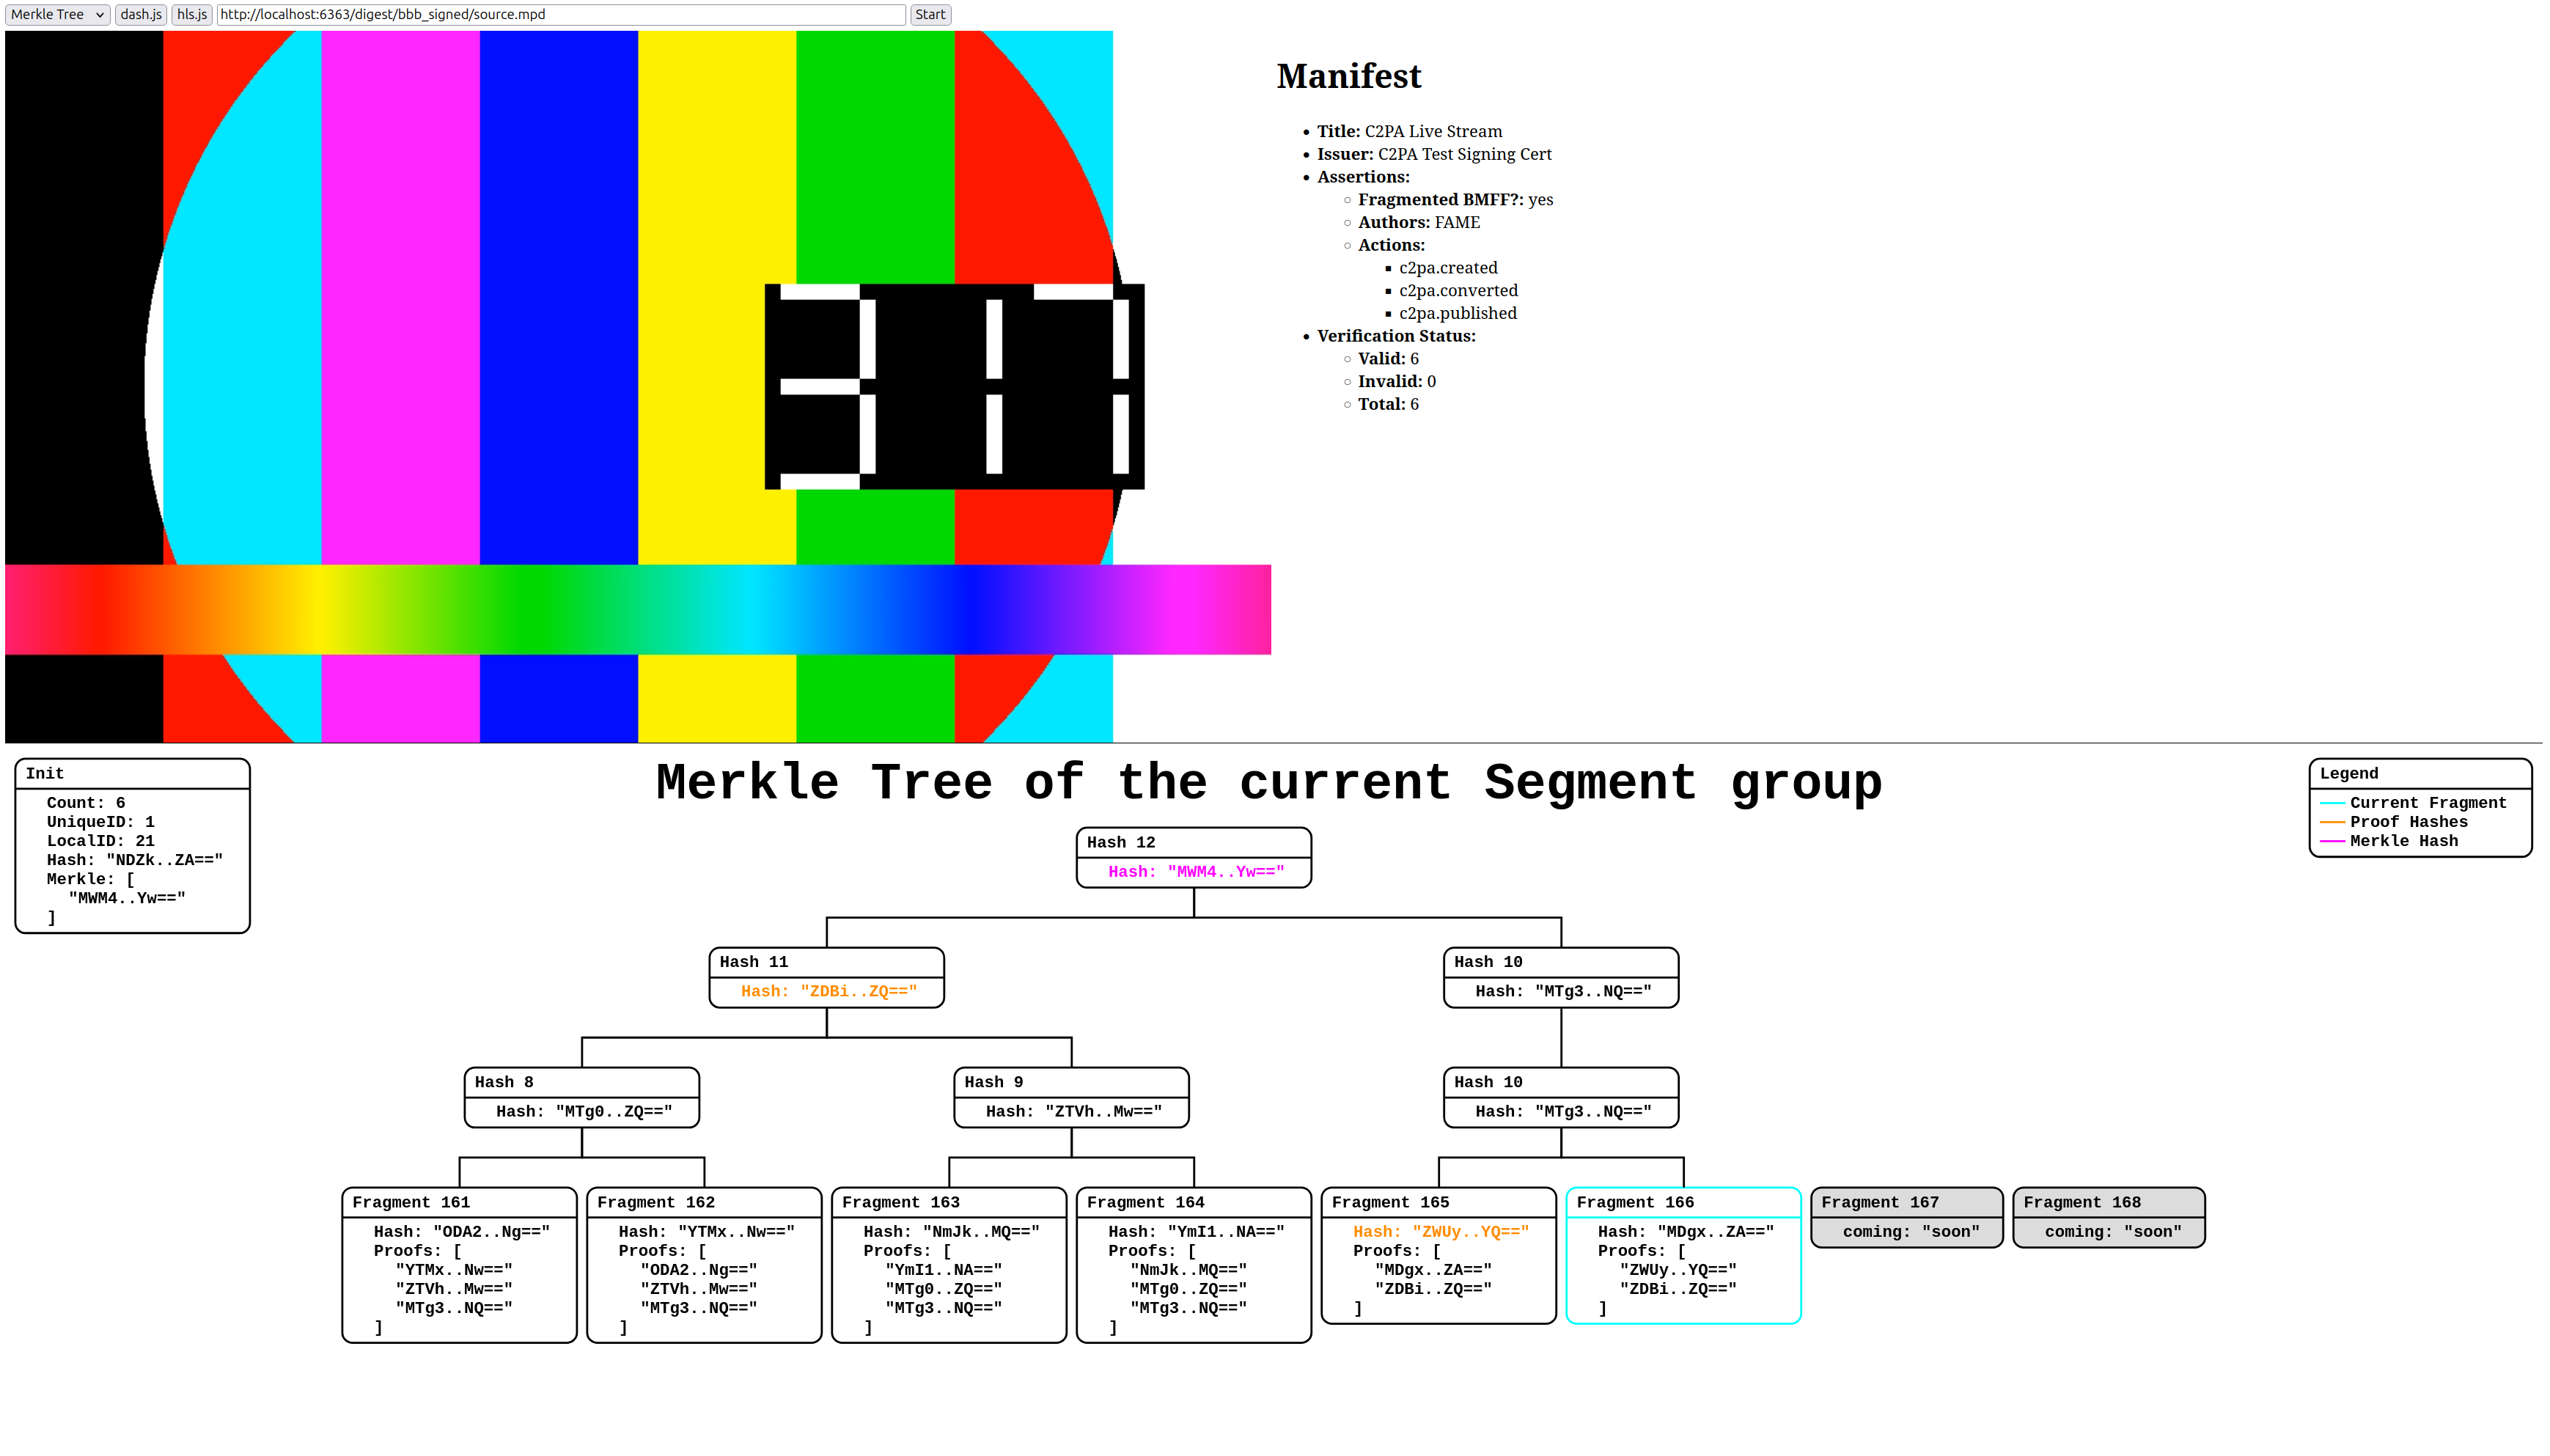
\includegraphics[width=0.95\linewidth, fbox]{merkle-tree-partial.png}
    \caption{Example Incomplete Merkle Tree Visualization}
    \label{fig:incomple_mt}
\end{figure}

\end{appendix}

\endinput


\end{document}
